\pdfoutput=1 % only if pdf/png/jpg images are used
\documentclass{JINST}

\usepackage{amsmath,amssymb}
\usepackage[numbers,sort]{natbib}
%\hypersetup{colorlinks, citecolor=blue, linkcolor=blue, filecolor=blue, urlcolor=red}

\title{Using a Magnetic Field to Improve Background Rejection in Neutrinoless Double Beta Decay Experiments Based in High Pressure Time Projection Chambers}

\author{J. Renner$^a$,\thanks{Corresponding author.}
J. J. Gomez-Cadenas$^a$,
D. Nygren$^b$, A. Cervera, J.A. Hernando, A. Imzaylov, F. Monrabal and J. Mu\~noz\\
\llap{$^a$}Instituto de F\'isica Corpuscular (IFIC), CSIC \& Universitat de Val\`encia,\\ 
Calle Catedr\'atico Jos\'e Beltr\'an, 2, 46980 Paterna, Valencia, Spain\\
\llap{$^b$}Name of Institute,\\
  Address, Country\\
E-mail: \email{CorrespondingAuthor@email.com}}

\bibliographystyle{unsrtnat}
%%%%%%%%%%%%%%%%%%%%%%%%%%%%%%%%%%%%%%%%%%%%%%%%%%
% $Id: commands.tex 1931 2015-01-17 10:32:50Z jmalbos $
% Some useful new commands...

%%%%%%%%%%%%%%%%%%%%%%%%%%%%%%%%%%%%%%%%%%%%%%%%%%
% BB
\newcommand{\bb}{\ensuremath{\beta\beta}}
% BB0NU
\newcommand{\bbonu}{\ensuremath{0\nu\beta\beta}}
% BB2NU
\newcommand{\bbtnu}{\ensuremath{2\nu\beta\beta}}

%%%%%%%%%%%%%%%%%%%%%%%%%%%%%%%%%%%%%%%%%%%%%%%%%%
% mBB
\newcommand{\mbb}{\ensuremath{m_{\bb}}}
% T0nu
\newcommand{\Tonu}{\ensuremath{T_{1/2}^{0\nu}}}
% Gonu
\newcommand{\Gonu}{\ensuremath{G^{0\nu}}}
% MNE
\newcommand{\Monu}{\ensuremath{\left|M^{0\nu}\right|}}
% Qbb
\newcommand{\Qbb}{\ensuremath{Q_{\bb}}}

%%%%%%%%%%%%%%%%%%%%%%%%%%%%%%%%%%%%%%%%%%%%%%%%%%
% kg·year
\newcommand{\kgy}{\ensuremath{\mathrm{kg}\cdot\mathrm{yr}}}
% Mbb
\newcommand{\Mbb}{\ensuremath{M_{\bb}}}
% kgbb
\newcommand{\kgbb}{\ensuremath{\mathrm{kg}_{\bb}}}
% ckky
\newcommand{\ckky}{\ensuremath{\mathrm{cts~keV^{-1}~kg^{-1}~yr^{-1}}}}
% ckkbby TO BE REVISED
\newcommand{\ckkbby}{\ckky}

%%%%%%%%%%%%%%%%%%%%%%%%%%%%%%%%%%%%%%%%%%%%%%%%%%
% Ca-48
\newcommand{\CA}{\ensuremath{^{48}\mathrm{Ca}}}
% Ge-76
\newcommand{\GE}{\ensuremath{^{76}\mathrm{Ge}}}
% Se-82
\newcommand{\SE}{\ensuremath{^{82}\mathrm{Se}}}
% Zr-96
\newcommand{\ZR}{\ensuremath{^{96}\mathrm{Zr}}}
% Mo-100
\newcommand{\MO}{\ensuremath{^{100}\mathrm{Mo}}}
% Pd-110
\newcommand{\PD}{\ensuremath{^{110}\mathrm{Pd}}}
% Cd-116
\newcommand{\CD}{\ensuremath{^{116}\mathrm{Cd}}}
% Sn-124
\newcommand{\SN}{\ensuremath{^{124}\mathrm{Sn}}}
% Te-130
\newcommand{\TE}{\ensuremath{^{130}\mathrm{Te}}}
% Xe-136
\newcommand{\XE}{\ensuremath{^{136}\mathrm{Xe}}}
% Nd-150
\newcommand{\ND}{\ensuremath{^{150}\mathrm{Nd}}}

% Ba-136
\newcommand{\BA}{\ensuremath{^{136}\mathrm{Ba}}}

% Tl-208
\newcommand{\TL}{\ensuremath{^{208}\mathrm{Tl}}}
% Bi-214
\newcommand{\BI}{\ensuremath{^{214}\mathrm{Bi}}}

\newcommand{\URANIUM}{Uranium}
\newcommand{\THORIUM}{Thorium}

% Xe-136
\newcommand{\NA}{\ensuremath{^{22}}Na}
\newcommand{\CS}{\ensuremath{^{137}}Cs}
\newcommand{\SEHF}{\ensuremath{\mathrm{SeF}_6}}
\newcommand{\COT}{\ensuremath{\mathrm{CO}_2}}
\newcommand{\CHF}{\ensuremath{\mathrm{CH}_4}}



%%%%%%%%%%%%%%%%%%%%%%%%%%%%%%%%%%%%%%%%%%%%%%%%%%
% W-values
\newcommand{\Wi}{\ensuremath{W_\mathrm{i}}}
\newcommand{\Wsc}{\ensuremath{W_\mathrm{sc}}}




%%%%%%%%%%%%%%%%%%%%%%%%%%%%%%%%%%%%%%%%%%%%%%%%%%


\abstract{We demonstrate that using an external magnetic field leads to an improved background rejection in neutrinoless double-beta (\bbonu) decay experiments based in high-pressure gas time projection chambers.  Such experiments are capable of imaging electron tracks, a feature that can be used to separate signal events (the two electrons emitted in a \bbonu\ decay) from background events, arising chiefly from single electrons of kinetic energy compatible with the end-point of the \bbonu\ decay (\Qbb) . Adding an external magnetic field of sufficiently high intensity (in the range of 0.5-1 Tesla for operating pressures in the range of 5-15 atmospheres), allows the measurement of the average sign of the electron(s) curvature in the gas. Such measurement is used  to construct an statistical estimator which can be used to reject background events by one order of magnitude at a moderate cost (60-80 \%) in efficiency signal. Combining this estimator with the excellent energy resolution and topological signature that can be obtained with high pressure gas TPCs it is possible to reach less than one count background event per ton year of exposure. Such low background rate is an essential feature of the next generation of \bbonu\ experiments, aiming to fully explore the inverse hierarchy of neutrino masses.}

\keywords{Neutrinoless double beta decay; magnetic field; TPC; high-pressure xenon chambers; ion chambers; Xenon; Selenium Hexafluoride.}


\begin{document}

\section{Introduction}\label{sec:intro}

Neutrinoless double beta decay (\bbonu) is a postulated very slow radioactive process in which two neutrons inside a nucleus transform into two protons emitting two electrons. The discovery of this process would demonstrate that neutrinos are Majorana particles and that total lepton number is not conserved in nature, two findings with far-reaching implications in particle physics and cosmology \cite{Gomez_2013,GomezCadenas:2013ue,Cadenas_2012}.

After 75 years of experimental effort, no compelling evidence for the existence of \bbonu\ decay has been obtained. If a discovery is not made by the current generation of \bbonu\ searches (see section \ref{sec:experiments} new experiments must be designed capable of simultaneously increasing the fiducial masses up to the ton scale, while reducing the backgrounds in the ROI by one to two orders of magnitude. A full exploration of the inverse hierarchy implies reaching sensitivities of 20 meV in the Majorana mass (section \ref{sec:boonu}). In turn, reducing the limit in \mbb\ by a factor five, requires reducing the limit in the \bbonu\ decay by a factor 25. This is a tremendous experimental challenge which requires to deploy masses in the ton scale, while reducing the backgrounds in the ROI to about {\em one or less} counts per ton of isotope mass and year. 

In this paper we show that a Magnetized Gaseous Experiment (MAGE) can, indeed reach a background rate of less than one count per ton of isotope and year of exposure. We discuss two different approaches. A magnetized High Pressure Xenon TPC, that we will call BEXT\footnote{Proposed by one of us (Gomez-Cadenas) an evolution of the NEXT experiment.}, and a magnetized ion Selenium TPC (MIST)\footnote{A novel concept, proposed by one of us (Nygren).} While BEXT is based in today's technology, MIST may require significant R\&D before it can be realized. However, if feasible, it would use of an important isotope (\SE) which at present is only being studied by the Super-NEMO demonstrator, which in turn uses a technology that cannot be extrapolated to large masses (e.g, ton scale). 

This paper is organized as follows. In section \ref{sec.bbonu} we briefly review the phenomenology of neutrinoless double beta decay. In ref{sec.bb} we summarize the state-of-the-art in \bbonu\ searches and show that background rates of less than one count per ton and year of exposure are needed in order to fully explore the so-called inverse hierarchy of neutrino masses with exposures in the range of the ton-year. In section \ref{sec:bext} we describe a conceptual design for BEXT. Section \ref{sec:MIST} presents MIST. In section 
\ref{sec.trk} we discuss tracking of electrons in a dense gas and show that a sufficiently intense magnetic field (in the range of 0.5 to 1 Tesla) combined with reasonably good resolution in the measurement of the track trajectory permits the determination of the {\em average sign of the electron(s)}, which can be used to discriminate between signal and background events. In section \ref{sec.results} we present the results of our Monte Carlo simulations.

 
%%%%%%%%%%%%%%%%%%%%%%%%%%%%%%%%%%%%%%%%%%%%%%%%%%%%%%%%%%%%
\section{Neutrinoless double beta decay and Majorana neutrinos}
\label{sec:bbonu}
%%%
Double beta (\bb) decay is a second-order weak process that transforms a nuclide of atomic number $Z$ into its isobar with atomic number $Z+2$. The ordinary decay mode consisting in two simultaneous beta decays (\bbtnu),
%%%
\begin{equation}
(Z,A) \to (Z+2,A) + 2~e^{-} + 2~\overline{\nu}_{e}\, ,
\end{equation}
%%%
The processes is suppressed in $G_F^2$, resulting in typical lifetimes of the order of $10^{18}$--$10^{21}$ years. With such long half-lives, for \bbtnu\ to be a competitive decay mode, the $\beta$ decay to the $Z+1$ nuclide must be either energetically forbidden or highly suppressed. Such a condition is fulfilled by 35 naturally-occurring isotopes thanks to the nuclear pairing force, which ensures that even-even nuclides are more bound than their odd-odd isobars.

The neutrinoless decay mode (\bbonu),
\begin{equation}
(Z,A) \rightarrow (Z+2,A) + 2\ e^{-}, \label{eq:bb0nu}
\end{equation}
violates total lepton number conservation, and is, therefore, forbidden in the Standard Model of particle physics. Its existence is linked to that of Majorana neutrinos. No convincing experimental evidence of the decay exists to date. 

Phase-space considerations alone would give preference to the \bbonu\ mode over the \bbtnu\ one, but the decay rate of the former is suppressed by the very small neutrino masses. In both decay modes the emitted leptons carry essentially all the available energy and the nuclear recoil is negligible. Therefore, in the \bbonu\ mode, the spectrum for the sum of the kinetic energies of the emitted electrons is a mono-energetic line at $\Qbb$, the $Q$ value of the reaction, defined as the mass difference between the parent and daughter nuclides:
%%%
\begin{equation}
Q_{\bb} \equiv M(A, Z) - M(A, Z+2).
\end{equation}
%%%
In the case of the \bbtnu-decay mode, the spectrum is continuous, extending from 0 to \Qbb\ and peaking below $\Qbb/2$.

%%%%%%%%%%
\begin{figure}
\centering
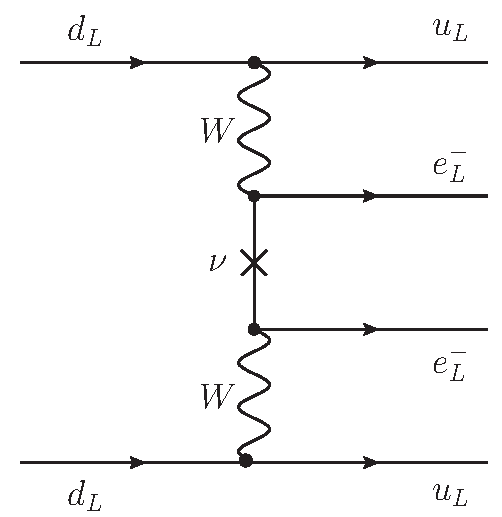
\includegraphics[scale=0.625]{img/LightNuExchange.pdf}
\caption{Neutrinoless double beta decay mediated by the standard mechanism, the virtual exchange of a light Majorana neutrino.} \label{fig:LightMajoranaNuExchange}
\end{figure}
%%%%%%%%%%

The standard mechanism responsible for the \bbonu\ decay is shown in Figure~\ref{fig:LightMajoranaNuExchange}.  The parent nucleus emits a pair of virtual $W$ bosons, and then these exchange a Majorana neutrino to produce the outgoing electrons. At the vertex where it is emitted, the exchanged neutrino is created, in association with an electron, as an antineutrino with almost total positive helicity, and only its small, $\mathcal{O}(m_{\nu}/E)$, negative-helicity component is absorbed at the other vertex. Considering that the amplitude is, in this case, a sum over the contributions of the three light neutrino mass states $\nu_i$ and is proportional to the square of the elements of the neutrino mixing matrix, $U_{ei}^2$, we conclude that the modulus of the amplitude for the \bbonu\ process must be proportional in this case to the \emph{effective neutrino Majorana mass}:
%%%
\begin{equation}
\mbb \equiv \left|\, \sum_{i=1}^3 U_{ei}^2\cdot m_i\ \right|, \label{eq:mbb}
\end{equation}
%%%
where $U_{ei}$ are the elements of the first row of the neutrino mixing matrix and $m_{i}$ are the three neutrino masses.

In the case where light Majorana neutrino exchange is the dominant contribution to \bbonu-decay, the inverse of the half-life for the process can be written as
%%%
\begin{equation}
\left(T^{0\nu}_{1/2}\right)^{-1} = G^{0\nu}\ \left|M^{0\nu}\right|^2\ \left(\frac{\mbb}{m_{e}}\right)^2.
\label{eq:Tonu}
\end{equation}
%%%
Here, \Gonu\ is a phase-space factor that depends on the transition $Q$ value and on the nuclear charge $Z$, and $M^{0\nu}$ is the nuclear matrix element (NME) for the process. The phase-space factor can be calculated analytically with sufficient accuracy (error estimates of about 1 per mille). The NME is evaluated using nuclear models, although with considerable uncertainty. In other words, the value of the effective neutrino Majorana mass, \mbb, can be inferred from a non-zero \bbonu-rate measurement, even though with some nuclear physics uncertainties. Conversely, if a given experiment does not observe the \bbonu\ process, the result can be interpreted in terms of an upper bound on \mbb.  

%%%%%%%%%%
\begin{figure}
\centering
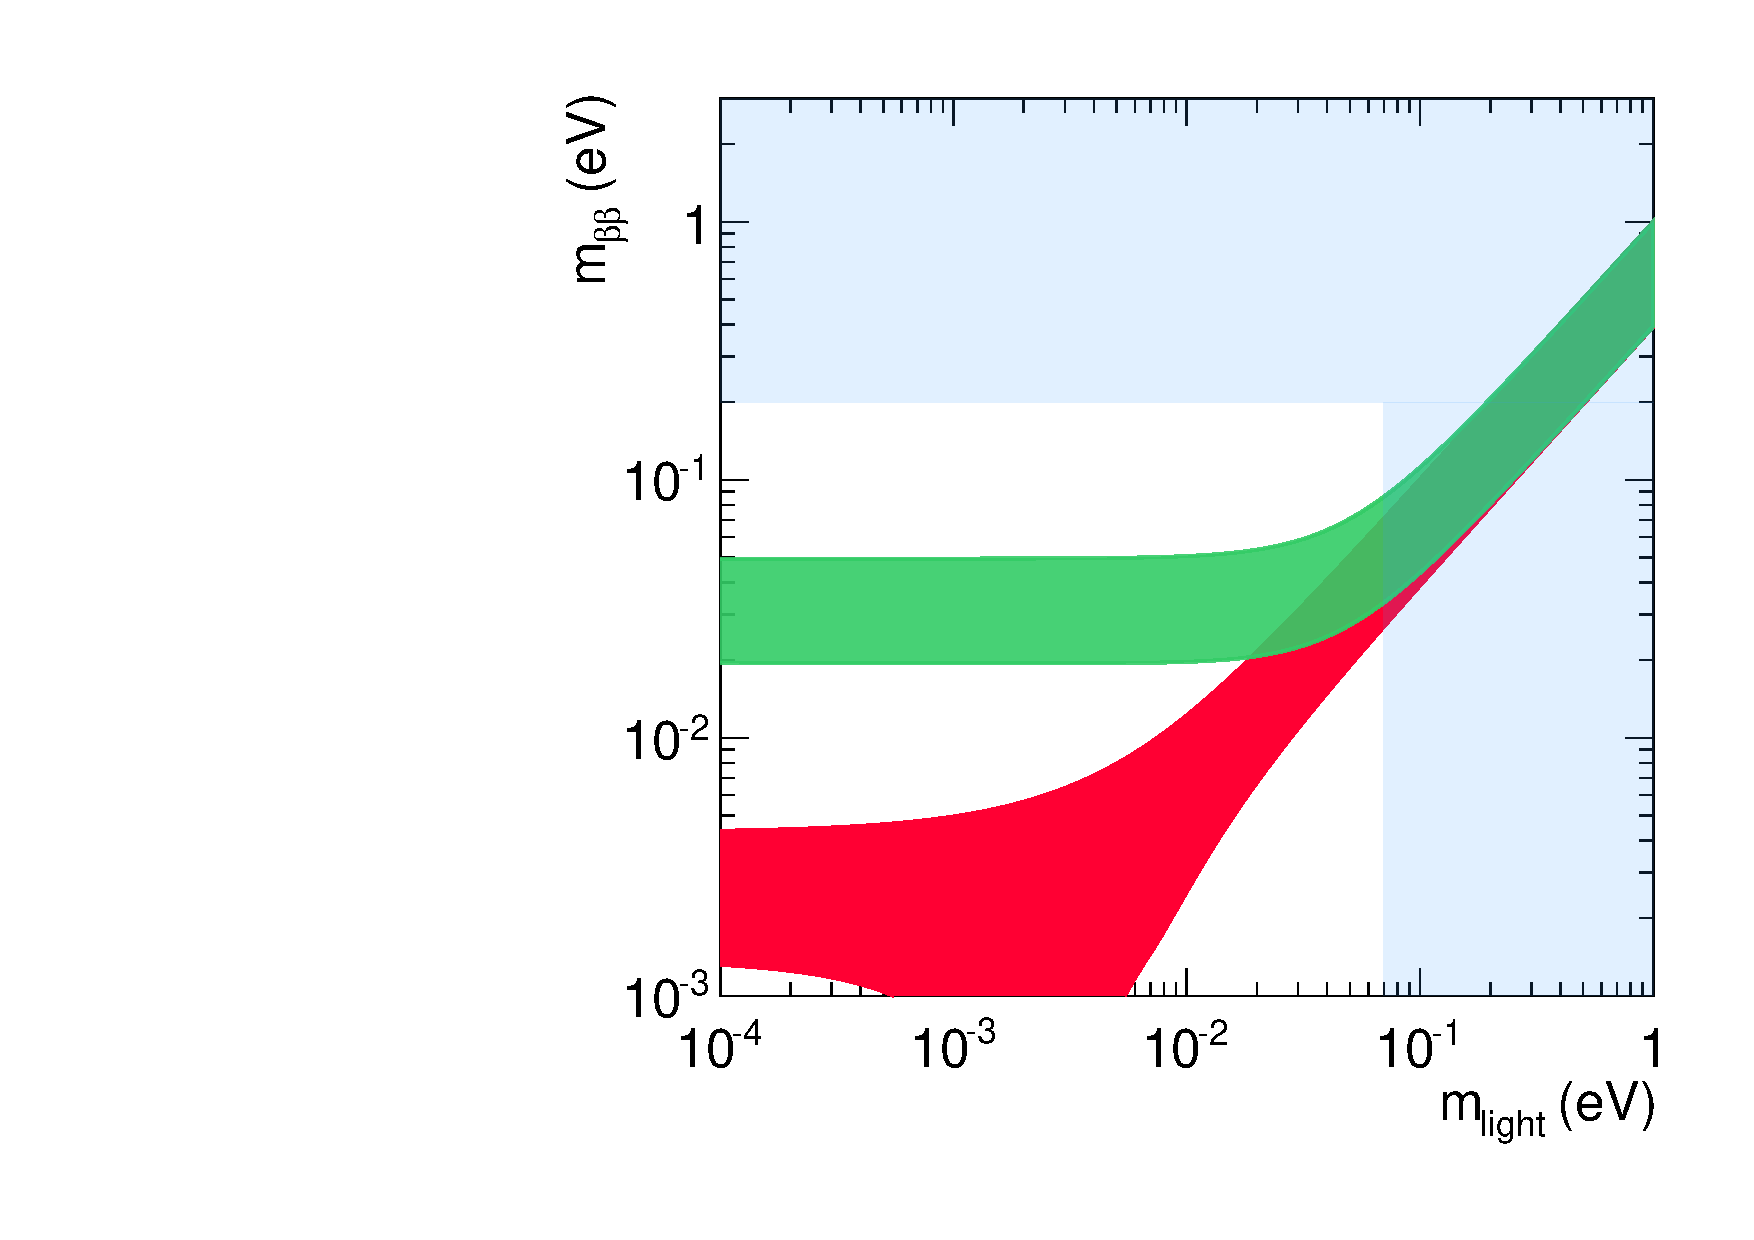
\includegraphics[width=0.525\textwidth]{img/BetaBetaVsLight.pdf}
\caption{The effective neutrino Majorana mass, \mbb, as a function of the lightest neutrino mass, $m_\mathrm{light}$. The green band corresponds to the inverted ordering of neutrino masses ($m_\mathrm{light}\equiv m_{3}$), while the red band corresponds to the normal ordering ($m_\mathrm{light}\equiv m_{1}$). The vertically-excluded region comes from cosmological bounds, while the horizontal one from \bbonu\ constraints.} \label{fig:BetaBetaVsLight}
\end{figure}


If light Majorana neutrino exchange is the dominant mechanism for \bbonu\ decay, it is clear from Eq.~(\ref{eq:mbb}) that the decay is then directly connected to neutrino oscillations phenomenology, and that it also provides direct information about the absolute neutrino mass scale. The relationship between \mbb\ and the actual neutrino masses $m_i$ is affected by the uncertainties in the measured oscillation parameters, the unknown neutrino mass ordering (normal or inverted) and the unknown phases in the neutrino mixing matrix (both Dirac and Majorana). For example, the relationship between \mbb\ and the lightest neutrino mass, $m_\mathrm{light}$, is shown in Figure~\ref{fig:BetaBetaVsLight}. The width of the two bands is due to the unknown CP violation phases and the uncertainties in the measured oscillation parameters. Figure \ref{fig:BetaBetaVsLight} also shows the upper bound on $m_\mathrm{light}$ from cosmology ($m_\mathrm{light}<0.07$ eV ), and an upper bound on \mbb\ from the current generation of \bbonu-decay searches ($m_{\beta\beta}<0.2$ eV ). See \cite{Gomez-Cadenas:2015twa} for a more detailed discussion and a full list of references). 

Notice that the current bounds on \mbb\ derived from GERDA-I, EXO-200 and KamLAND-ZEN, are of the order of $\mbb < 200$~meV, while the cosmological bounds on m$_{light}$~are of the order of
$m_{light} < 100$~meV. By $\sim$ 2020, The ``current generation'' of \bbonu\ experiments (including GERDA-II, {\scshape Majorana}, NEXT, CUORE, SNO+  and the SuperNEMO demonstrator, as well as upgrades of KamLAND-ZEN and EXO-200) will, probably, be able to push the current sensitivity to about $\mbb < 50-100$~meV. If a discovery is not made, then, the current generation of \bbonu\ experiments will exclude the so-called ``degenerated hierarchy'' ($m_1 \sim m_2 \sim m_3$) of neutrino masses. The goal of the ``next generation'' of \bbonu\ experiments is to fully explore the inverse hierarchy (green band in the figure, $\mbb < 20$~meV.)

%%%%%%%%%%

\section{The experimental effort}\label{sec:experiments}

During the last decade the field of \bbonu\ searches has exploded. Three experiments (EXO-200 \cite{Albert:2014awa, Auger:2012ar}, KamLAND-Zen \cite{Asakura:2014lma, Gando:2012zm} and GERDA-I \cite{Agostini:2013mzu}) have released physics results, excluding  lifetimes below $10^{25}$~years for the \bbonu\ of \XE\ (EXO-200 and KamLAND-Zen) and the \bbonu\ mode of \GE\ (GERDA-I). 
Five more experiments will start operations in the next few years.  {\scshape Majorana} \cite{Abgrall:2013rze}(germanium diodes), NEXT-100 \cite{Gomez-Cadenas:2014dxa} (a high-pressure gas xenon TPC), CUORE  \cite{Giachero:2014hva} (TeO$_{2}$ crystal bolometers), SNO+ \cite{Biller:2014eha} (Tellurium  dissolved in liquid scintillator) and the SuperNEMO demonstrator \cite{Guzowski:2014ina} (using Selenium). We refer to all these as the
``current generation'' of \bbonu\ searches. The typical exposures deployed will be of the order of 20 kg $\cdot$yr for the SuperNEMO demonstrator, 50--100 kg $\cdot$yr for germanium experiments (GERDA and  {\scshape Majorana} ), 300 kg $\cdot$yr for the xenon TPCs (EXO-200 and NEXT-100), and around 500 kg $\cdot$yr for CUORE, SNO+ and KamLAND-ZEN. The expected background in the ROI (measured in the case of 
EXO-200, KamLAND-Zen and GERDA-I, computed by Monte Carlo calculations for all the others) varies between $\sim$10 and $\sim$ 100 events per ton and year. The expected sensitivity to the Majorana neutrino mass (\mbb), after some 3 years run, of several of these experiments is in the range of 100 meV \cite{Gomez-Cadenas:2015twa}.

The performance of the various experiments can be summarized in terms of their basic operational parameters. These are: a) the \bb\ source isotope; b) the energy resolution $\Delta E$ (usually expressed as FWHM); the specific background rate ($c$) in the region of interest (ROI) around \Qbb (normally expressed in \ckky); the signal detection efficiency, $\varepsilon$; and the source mass M. The exposure is obtained multiplying the source mass by the running time. 

%The basic operational parameters of the experiments of the current generation are listed in Table~\ref{tab:ParamsCurrentGeneration}. The size of the uncertainties associated to the parameters varies according to the state of development of each project.  The smallest uncertainties correspond to the running experiments, which have \emph{measured} their operational parameters. CUORE and GERDA-II have assessed their expected performance with setups operating under conditions similar to those of the final experiment. The remaining experiments base their expectations on results obtained with R\&D prototypes, ancillary measurements and Monte Carlo simulations. 
%
%%%%%%%%%%%
%\begin{table}[!]
%\centering
%\caption{Basic operational parameters of the \bbonu-decay experiments of the current generation: \bb\ source isotope, energy resolution (FWHM), $\Delta E$; background rate in the region of interest around \Qbb; signal detection efficiency, $\varepsilon$; and source mass.} \label{tab:ParamsCurrentGeneration}
%\small
%\begin{tabular*}{\textwidth}{@{\extracolsep{\fill}} l c D{.}{.}{3.0} D{.}{.}{0.5} c D{.}{.}{3.0}}
%\toprule
%Experiment & Isotope & \multicolumn{1}{c}{$\Delta E$} & \multicolumn{1}{c}{Bkgnd.\ rate} & \multicolumn{1}{c}{$\varepsilon$} & \multicolumn{1}{c}{Mass} \\
%           &         & \multicolumn{1}{c}{(keV)} & \multicolumn{1}{c}{(keV$^{-1}$~kg$^{-1}$~yr$^{-1}$)} & \multicolumn{1}{c}{$(\%)$} & \multicolumn{1}{c}{(kg)} \\ \midrule
%%
%CUORE-0\hair\textsuperscript{\itshape a} \cite{Giachero:2014hva} & \TE\ & 5 & 0.23 & 78 & 11 \\
%%
%CUORE\hair\textsuperscript{\itshape b} \cite{Alessandria:2011rc} & \TE\ & 5 & 0.04 & 87 & 206 \\
%%
%GERDA-I\hair\textsuperscript{\itshape a} \cite{Agostini:2013mzu} & \GE\ &   5 & 0.013 & 62 & 15 \\
%%
%GERDA-II\hair\textsuperscript{\itshape b} \cite{Macolino:2014vya} & \GE\ & 3 & 0.001 & 66 & 33 \\
%%
%EXO-200\hair\textsuperscript{\itshape a} \cite{Albert:2014awa} & \XE\ & 88 & 0.002 & 85 & 76 \\
%%
%KamLAND-Zen\hair\textsuperscript{\itshape a} \cite{Gando:2012zm, Asakura:2014lma} & \XE\ & 243 & 0.00014  & 25 & 348 \\
%%
%{\scshape Majorana}\textsuperscript{\itshape c} \cite{Abgrall:2013rze} & \GE\ & 4 & 0.0009 & 70 & 25 \\
%%
%NEXT-100\hair\textsuperscript{\itshape c} \cite{Gomez-Cadenas:2014dxa} & \XE\ &  17 & 0.0005  & 30 & 91 \\
%%
%SNO+\hair\textsuperscript{\itshape c} \cite{Biller:2014eha} & \TE\ & 264 & 0.0001  & 15 & 800 \\
%%
%SuperNEMO-D\hair\textsuperscript{\itshape c} \cite{Guzowski:2014ina} & \SE\ & 120 & 0.0005 & 30 & 7 \\ 
%%%
%\bottomrule \\[-8pt]
%%
%\multicolumn{6}{l}{\textsuperscript{\itshape a} \footnotesize The experiment is running and has measured its operational parameters.} \\[-2pt]
%\multicolumn{6}{l}{\textsuperscript{\itshape b} \footnotesize The experiment has proven its feasibility with a demonstrator.} \\[-2pt]
%\multicolumn{6}{l}{\textsuperscript{\itshape c} \footnotesize The operational parameters are estimations based on R\&D results and simulations. } \\
%\end{tabular*}
%\end{table}
%%%%%%%%%%%

The total background in the ROI per year $b$ is readily obtained as $b = c \cdot M \cdot t \cdot \Delta E$. The sensitivity to the Majorana neutrino mass of a background free experiment improves with the square root of the exposure. Contrarily, in the limit of background--limited experiments, the sensitivity of \bbonu\ experiments can be approximated by (see discussion in \cite{Gomez-Cadenas:2015twa}):

\begin{equation}
{S}(\mbb) = \propto \sqrt{1/\varepsilon}\ \left(\frac{c~\Delta E}{M~t}\right)^{1/4}\,. \label{eq:Sensitivity3}
\end{equation}
%%%

Since the background limits dramatically the sensitivity of a double beta decay experiment, any extrapolation of scale requires a huge effort. For example, the NEXT-100 experiment foresees to reach a sensitivity of 
$\mbb < 100$~meV for an exposure of 300 kg $\cdot$ year and a background rate of $\sim$1 count per 100 kg and year in the ROI. For an exposure of 1 ton $\cdot$ year, NEXT-100 would register about 10 background counts per year in the ROI and its sensitivity would be in the background-dominated regime. To explore the inverse hierarchy it is necessary to reach $\mbb < 20$~meV. Upgrading the NEXT detector by simply building a detector or larger mass (without adding an improvement to the technology that would drastically reduce the background) would not work, since in the background-dominated regime, an improvement of a factor 5 in $\mbb$ requires an improvement of 625 in the product $b/E$. Thus, if $b$~ does not improve, the total exposure would approach some 200 tons $\cdot$ year. Unfortunately, even assuming a very long running period, say of 10 years, building a 20 ton high pressure xenon chamber appears difficult. 

On the other hand, the HPXe technology should permit to reach a resolution of at least 0.5 \% FWHM at \Qbb\ \cite{Alvarez:2012kua}, thus reducing the ROI to some 12 keV. Even more important, as we will show in this paper, adding a magnetic field to NEXT could reduce the specific background in the ROI to about $5 \times 10^{-5}$~ \ckky. Then, $b \sim 0.6$ counts per year and ton and the upgraded experiment would be in the background-free regime. Therefore to improve the sensitivity to $\mbb$~by a factor 5, one needs to reduce $b/E$~by ``only'', a factor 25, which in turn translates in a ``moderate'' exposure of some 2 ton $\cdot$ year. 


%%%%%%%%%%
\begin{figure}
\centering
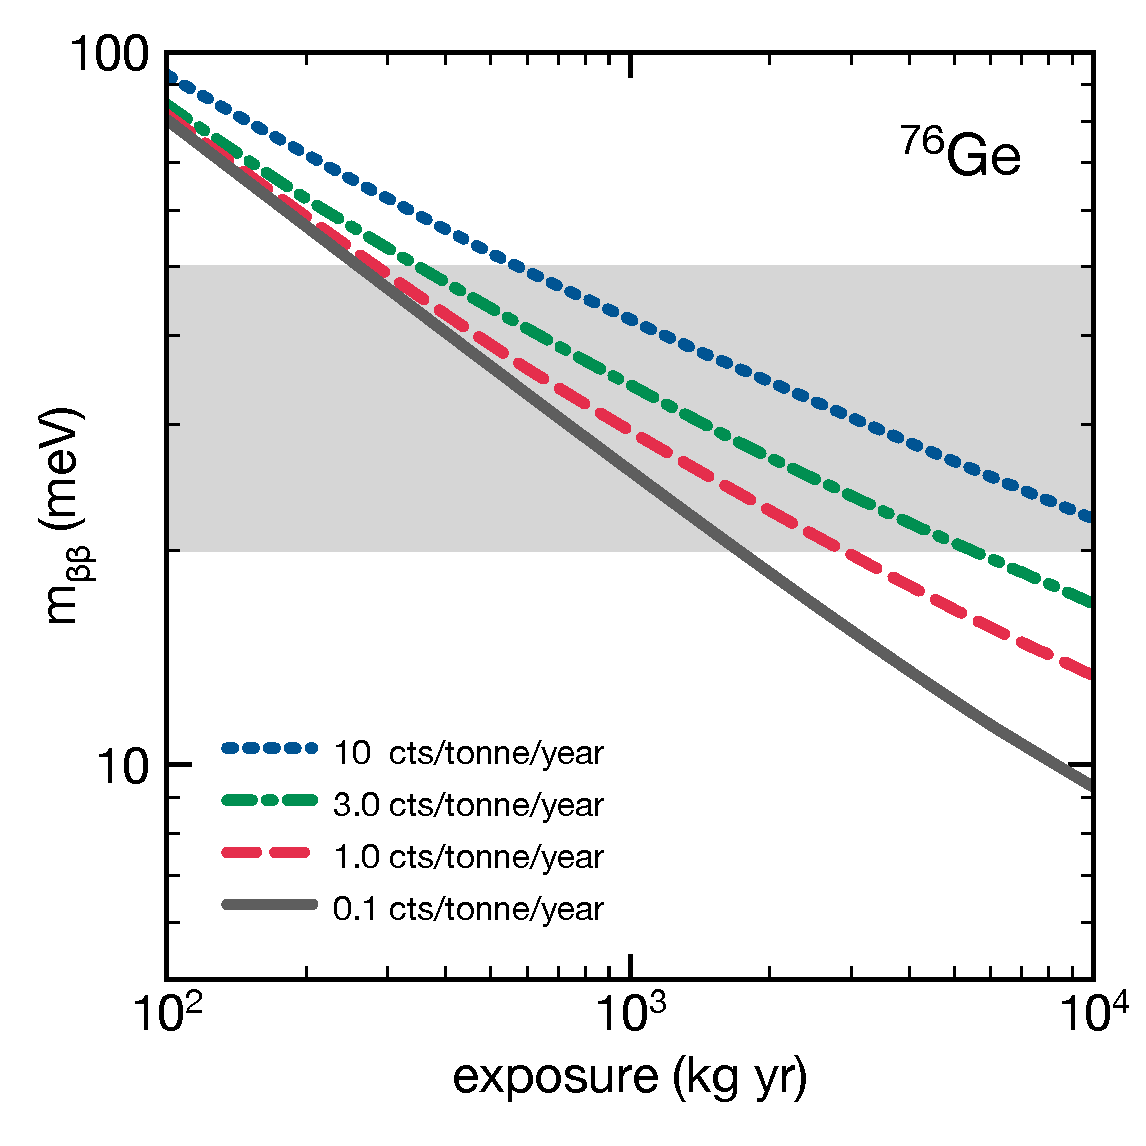
\includegraphics[width=0.45\textwidth]{img/FutureGe76.pdf}
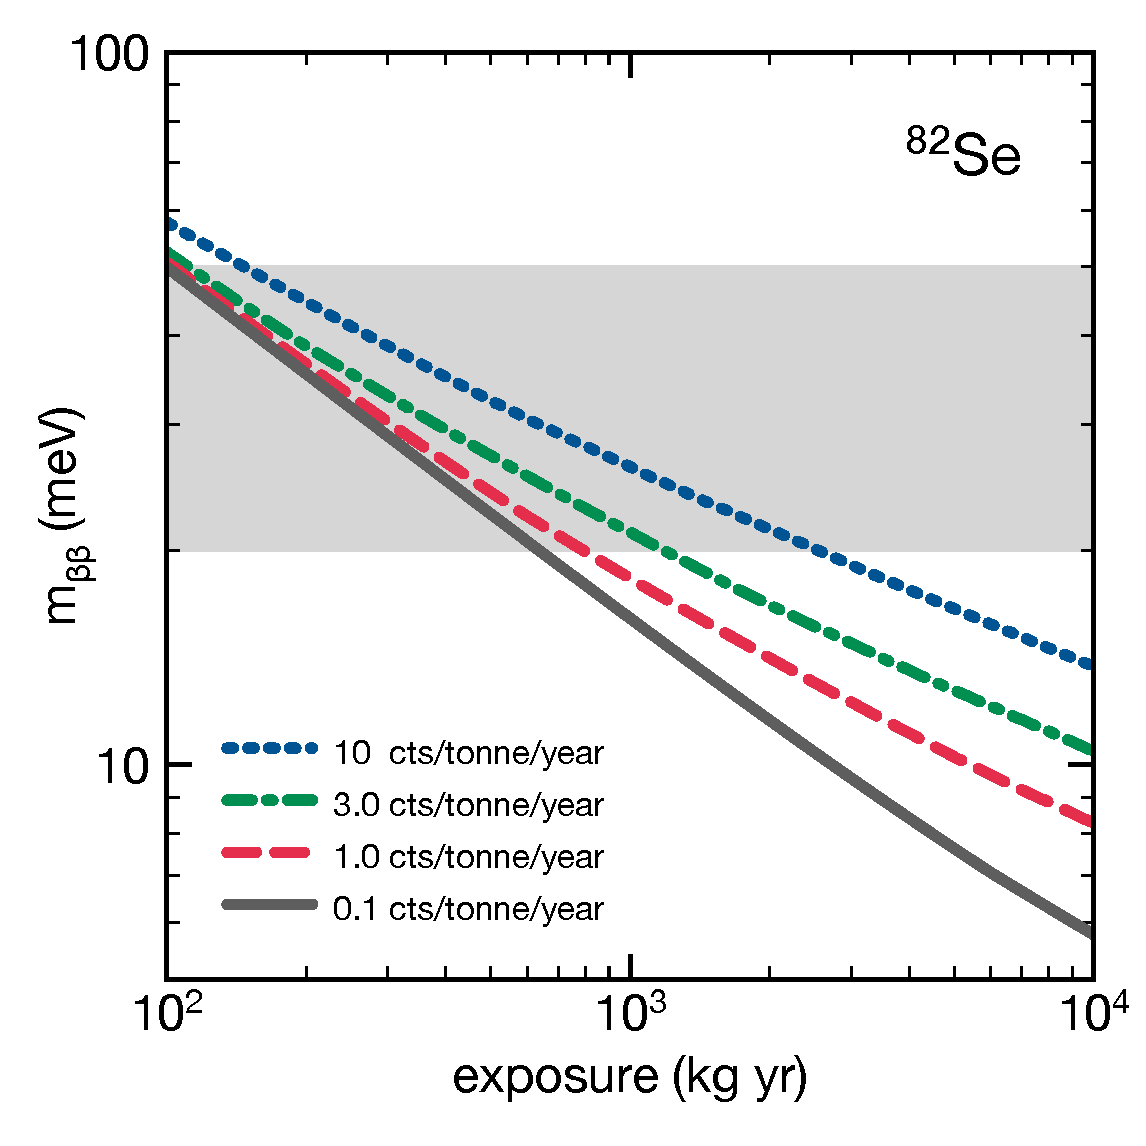
\includegraphics[width=0.45\textwidth]{img/FutureSe82.pdf}
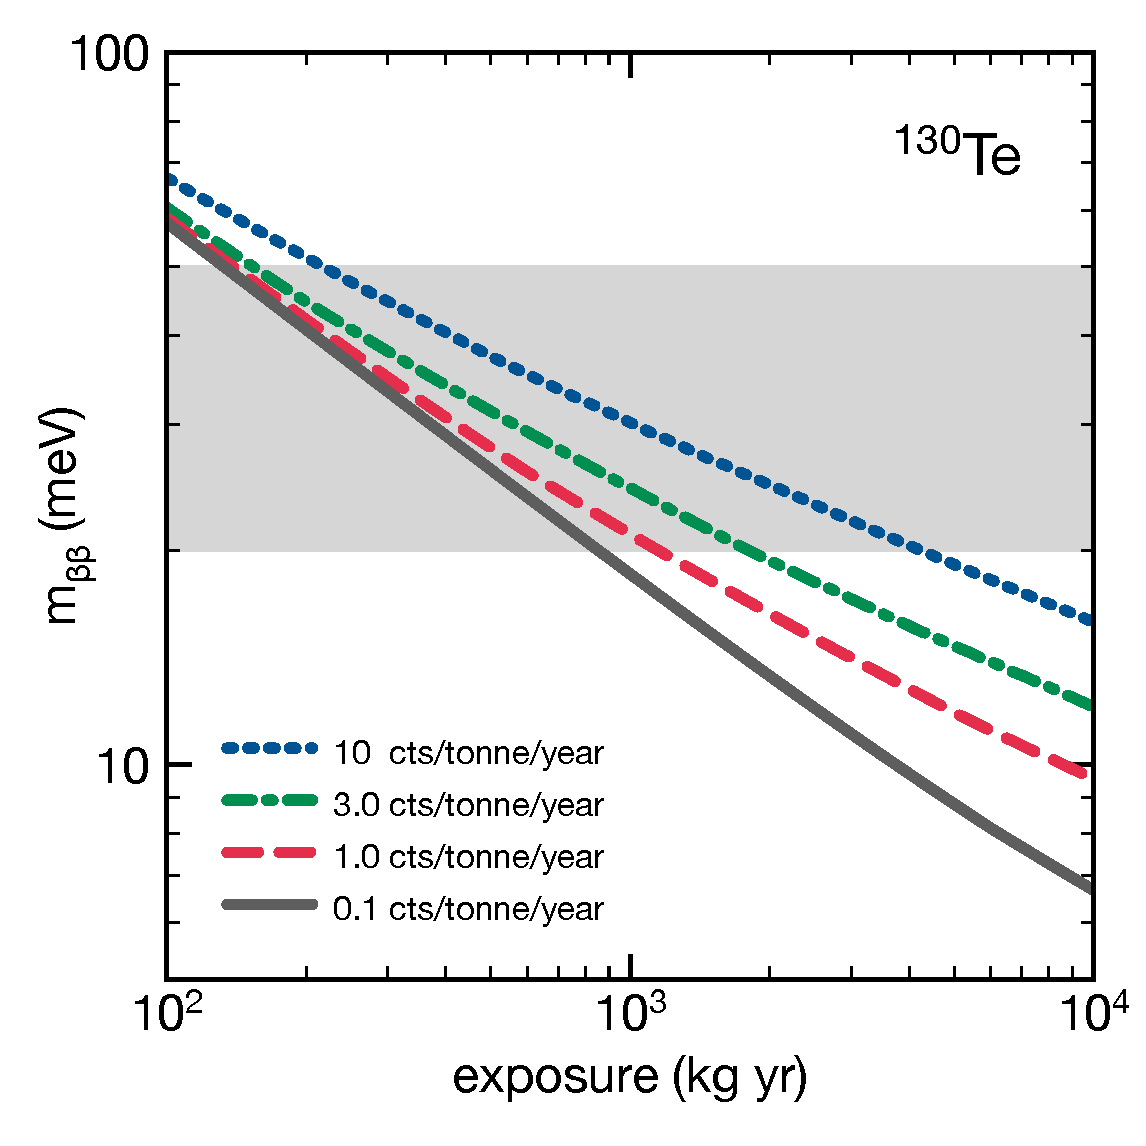
\includegraphics[width=0.45\textwidth]{img/FutureTe130.pdf}
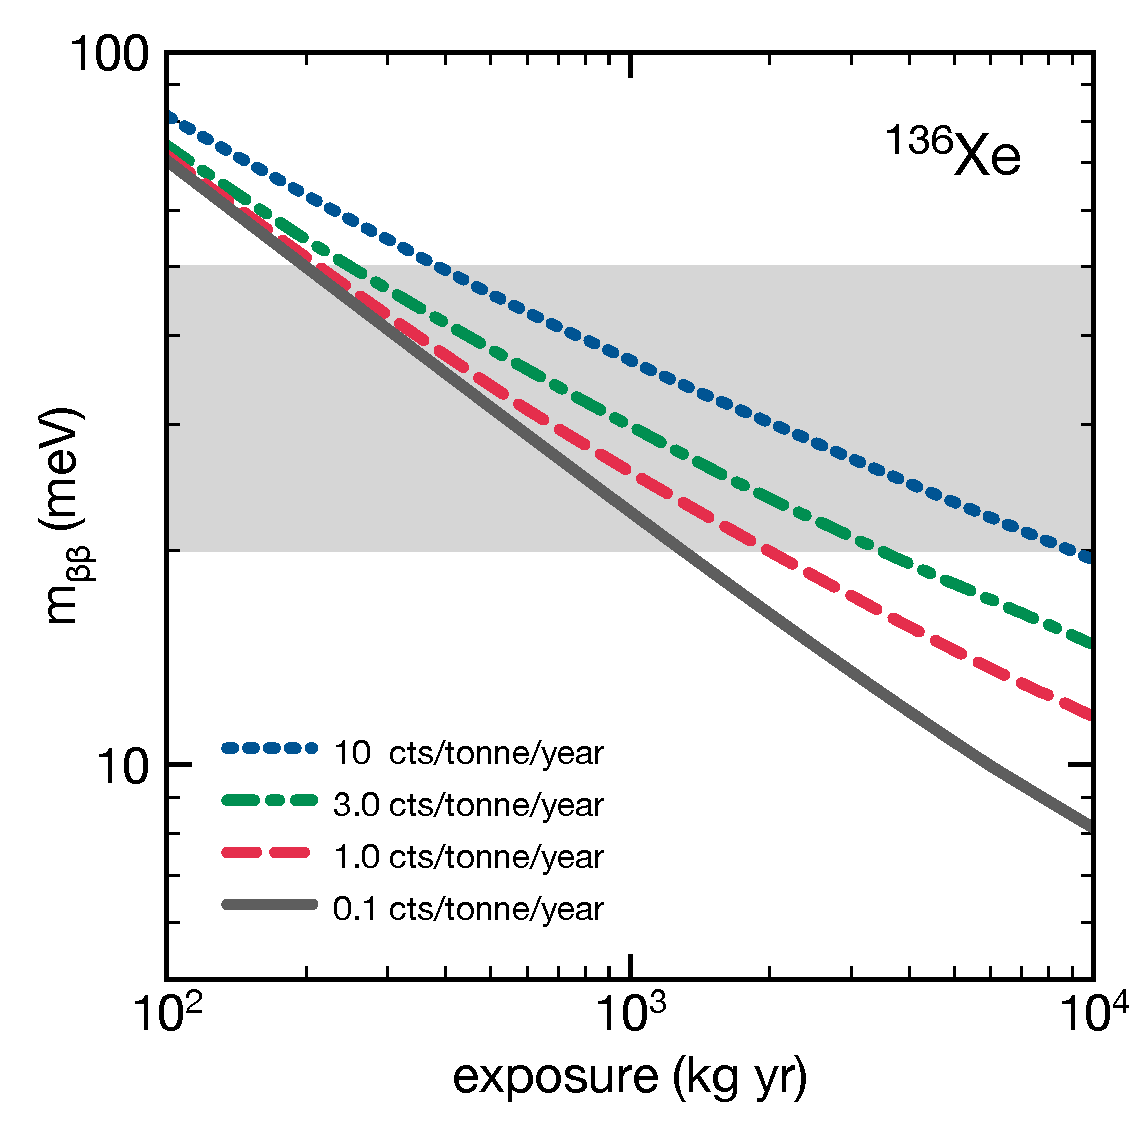
\includegraphics[width=0.45\textwidth]{img/FutureXe136.pdf}
\caption{Exposure dependence of the \mbb\ sensitivity (at 90\% CL) of perfectly-efficient experiments based on 4 different isotopes and with 4 different assumptions for the background rate in the ROI. The grey band represents the inverted-hierarchy region of neutrino masses.} \label{fig:FutureGen}
\end{figure}
%%%%%%%%%%

Figure \ref{fig:FutureGen} quantifies the above discussion, showing the exposure dependence of the \mbb\ sensitivity (at 90\% CL) of perfectly-efficient experiments based on 4 different isotopes and with 4 different assumptions for the background rate in the ROI. Notice that the grey band represents the inverted-hierarchy region of neutrino masses. If perfectly efficient, the putative NEXT upgraded detector that we have just described, with a background rate of 0.6 counts per ton and year would cover the inverted hierarchy with an exposure of less than 2 ton $\cdot$~year. Including a realistic efficiency (in the range of 30\%), would push the required exposure to some 6 ton $\cdot$ year, reachable with a detector deploying a fiducial mass of around one ton of isotope.  


\section{NEXT: A HPXe TPC}
%%%

%%%%%%%%%%
\begin{figure}
\centering
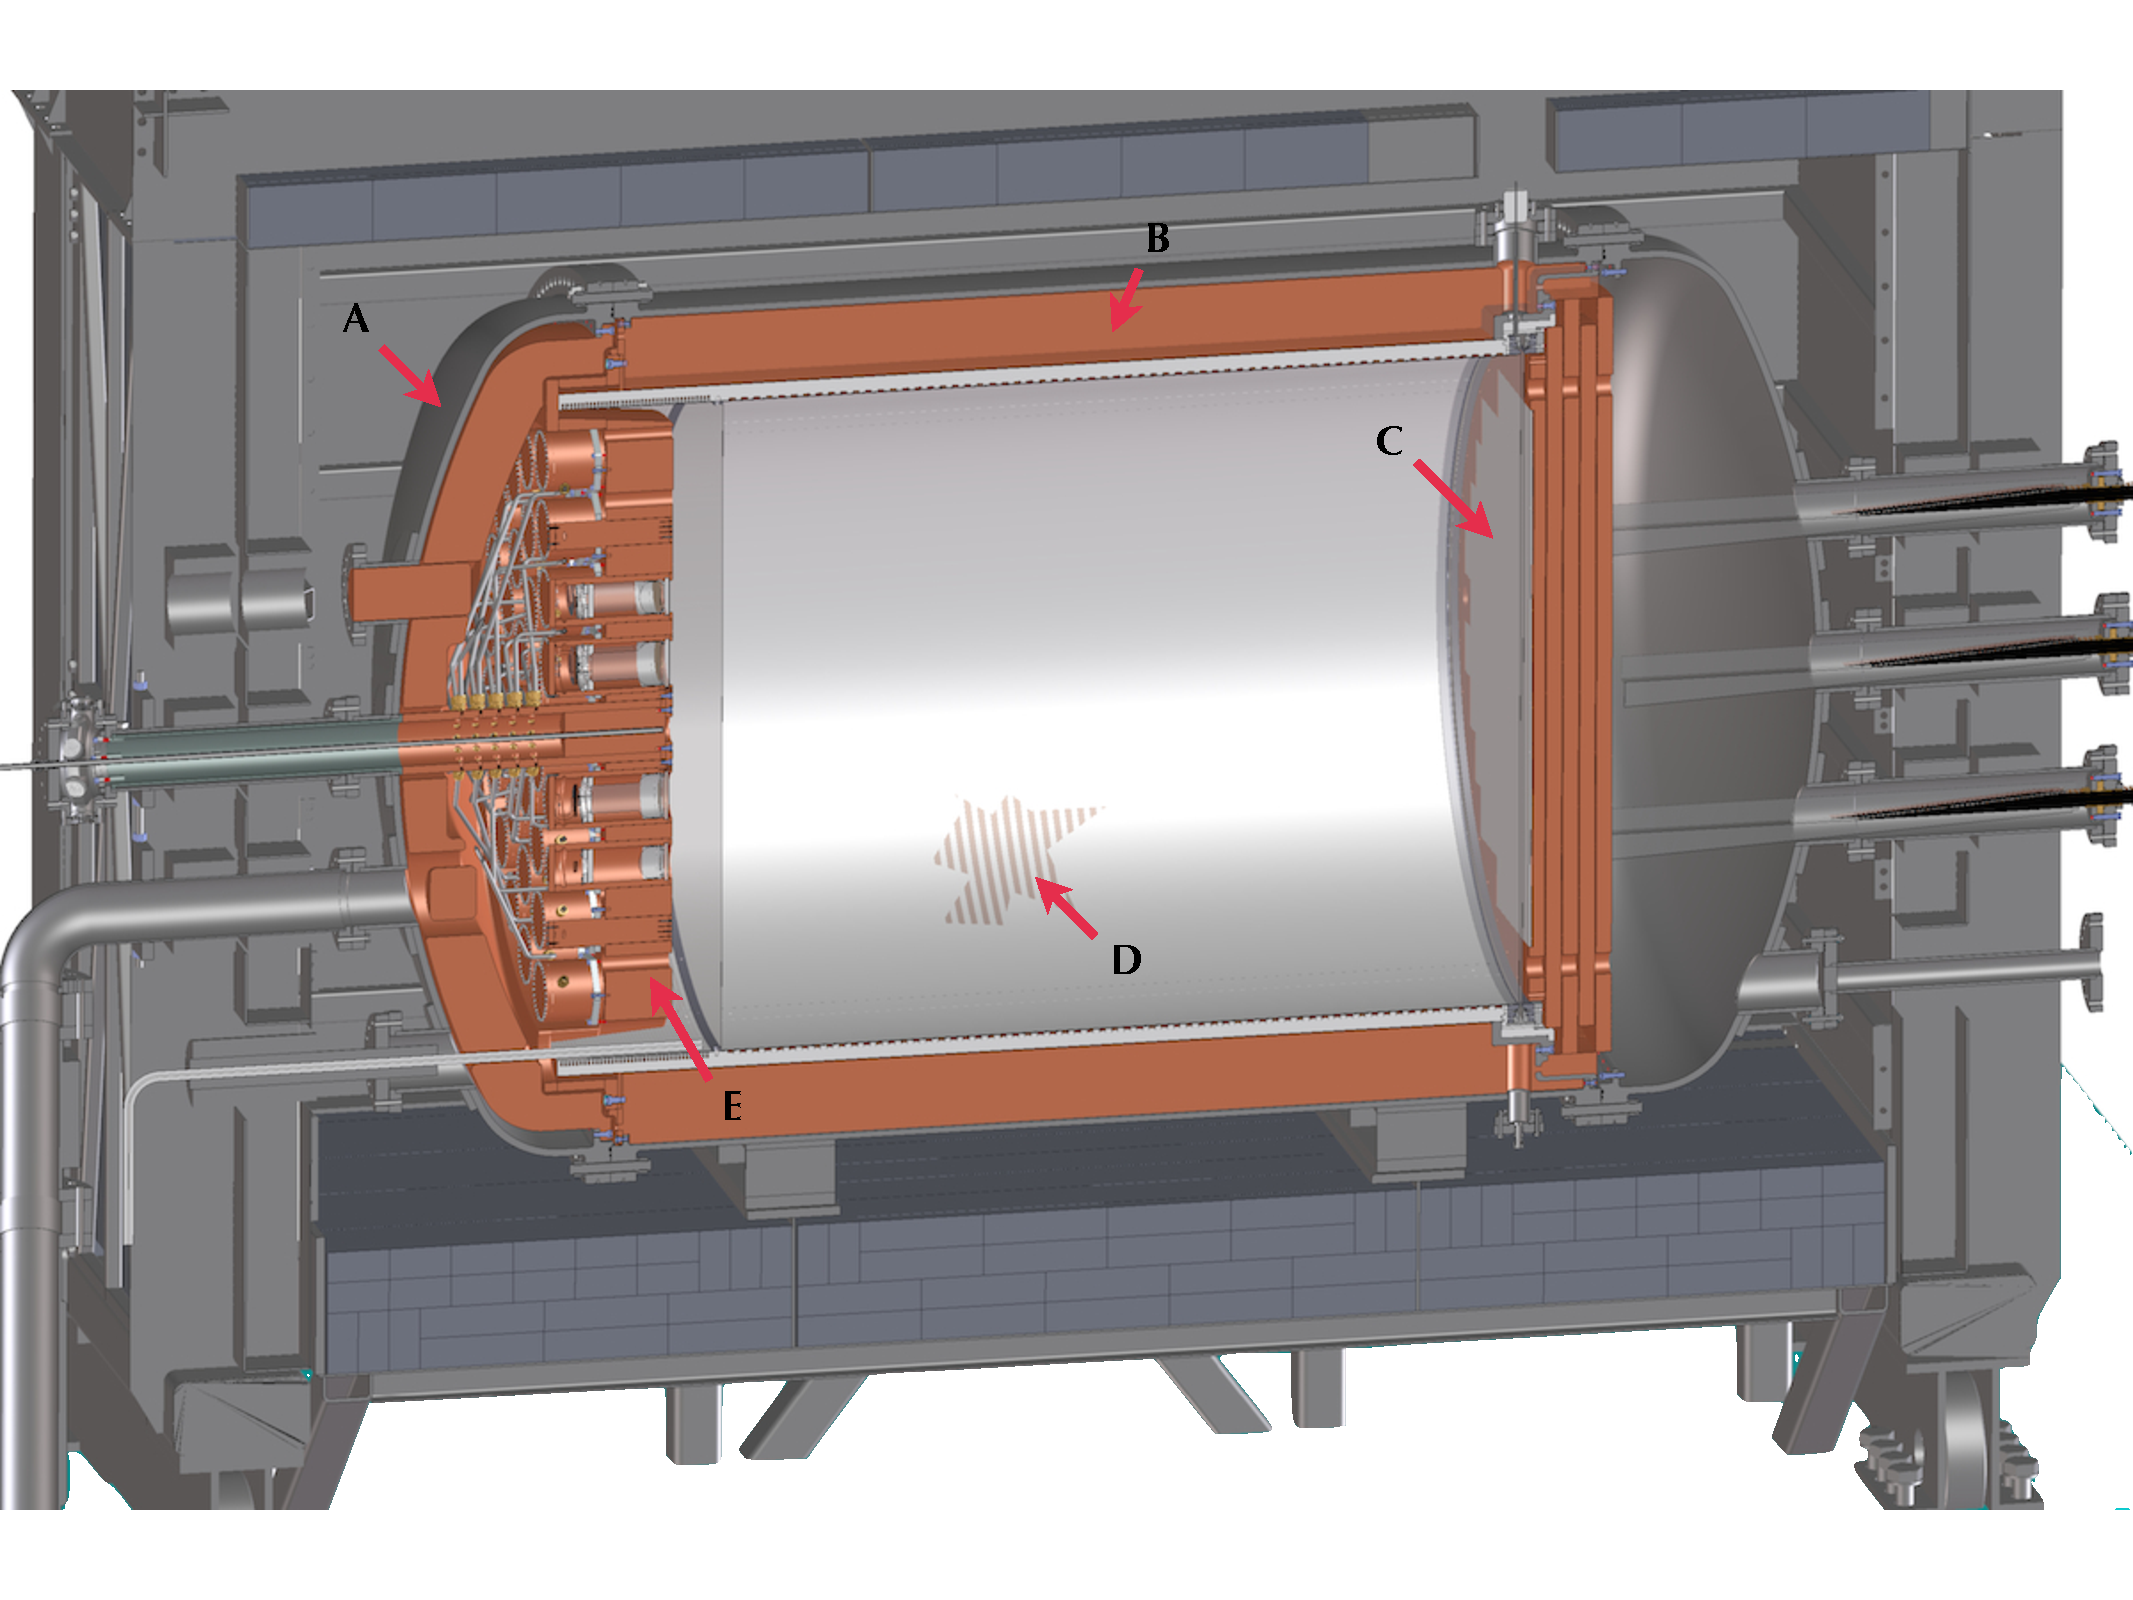
\includegraphics[width=0.9\textwidth]{img/Next100.pdf}
\caption{A cross-section drawing of the NEXT-100 detector. The pressure vessel (A) is made of stainless steel Grade 316Ti, and its dimensions are 130~cm inner diameter, 222~cm length and 1~cm thick walls, for a total mass of 1\,200 kg. The inner copper shield (B) is made of ultra-pure copper bars and is 12~cm thick, with a total mass of 9\,000 kg. The time projection chamber (D) includes the field cage, cathode, EL grids and HV penetrators. The light tube is made of thin teflon sheets coated with TPB (a wavelength shifter). The energy plane (E) is made of 60 PMTs housed in copper enclosures. The tracking plane (C) is made of MPPCs arranged into 8$\times$8 boards.} \label{fig.NEXT100}
\end{figure}
%%%%%%%%%%

The \emph{Neutrino Experiment with a Xenon TPC} (NEXT) \cite{Gomez-Cadenas:2013lta} will search for the neutrinoless double beta decay of \XE\ using a high-pressure xenon gas time projection chamber. The design of the NEXT-100 detector (Figure \ref{fig.NEXT100}) is optimised for energy resolution by using proportional electroluminescent (EL) amplification of the ionisation signal. The detection process involves the use of the prompt scintillation light from the gas as start-of-event time, and the drift of the ionisation charge to the anode by means of an electric field ($\sim0.3$ kV/cm at 15 bar) where secondary EL scintillation is produced in the region defined by two highly transparent meshes, between which there is a field of $\sim20$ kV/cm at 15 bar. The detection of EL light provides an energy measurement using photomultipliers (PMTs) located behind the cathode (the \emph{energy plane}) as well as tracking through its detection a few mm away from production at the anode, via a dense array of silicon photomultipliers (the \emph{tracking plane}).

\begin{figure}
\centering
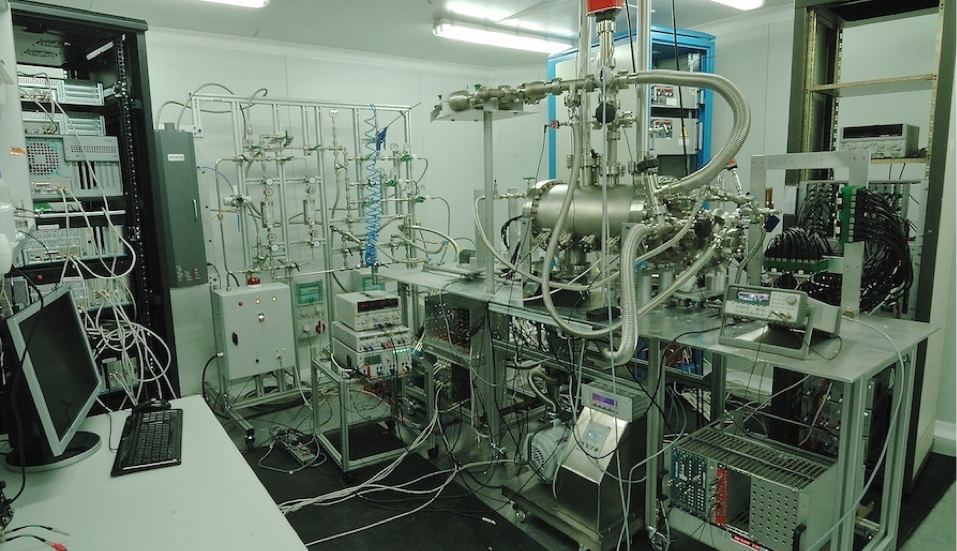
\includegraphics[width=0.9\textwidth]{img/DemoSetup.png}
\caption{\small The NEXT-DEMO setup at IFIC (Valencia, Spain).} \label{fig.DEMO}
\end{figure}

The R\&D phase of the experiment was carried out with the large-scale prototypes NEXT-DEMO (shown in Figure \ref{fig.DEMO}) and NEXT-DBDM. The prototypes have measured excellent energy resolution, extrapolating to 0.5--0.7 \% FWHM at \Qbb\  \cite{Alvarez:2012xda,Alvarez:2012kua,Lorca:2014sra}. 

%%%%%
\begin{figure}
\centering
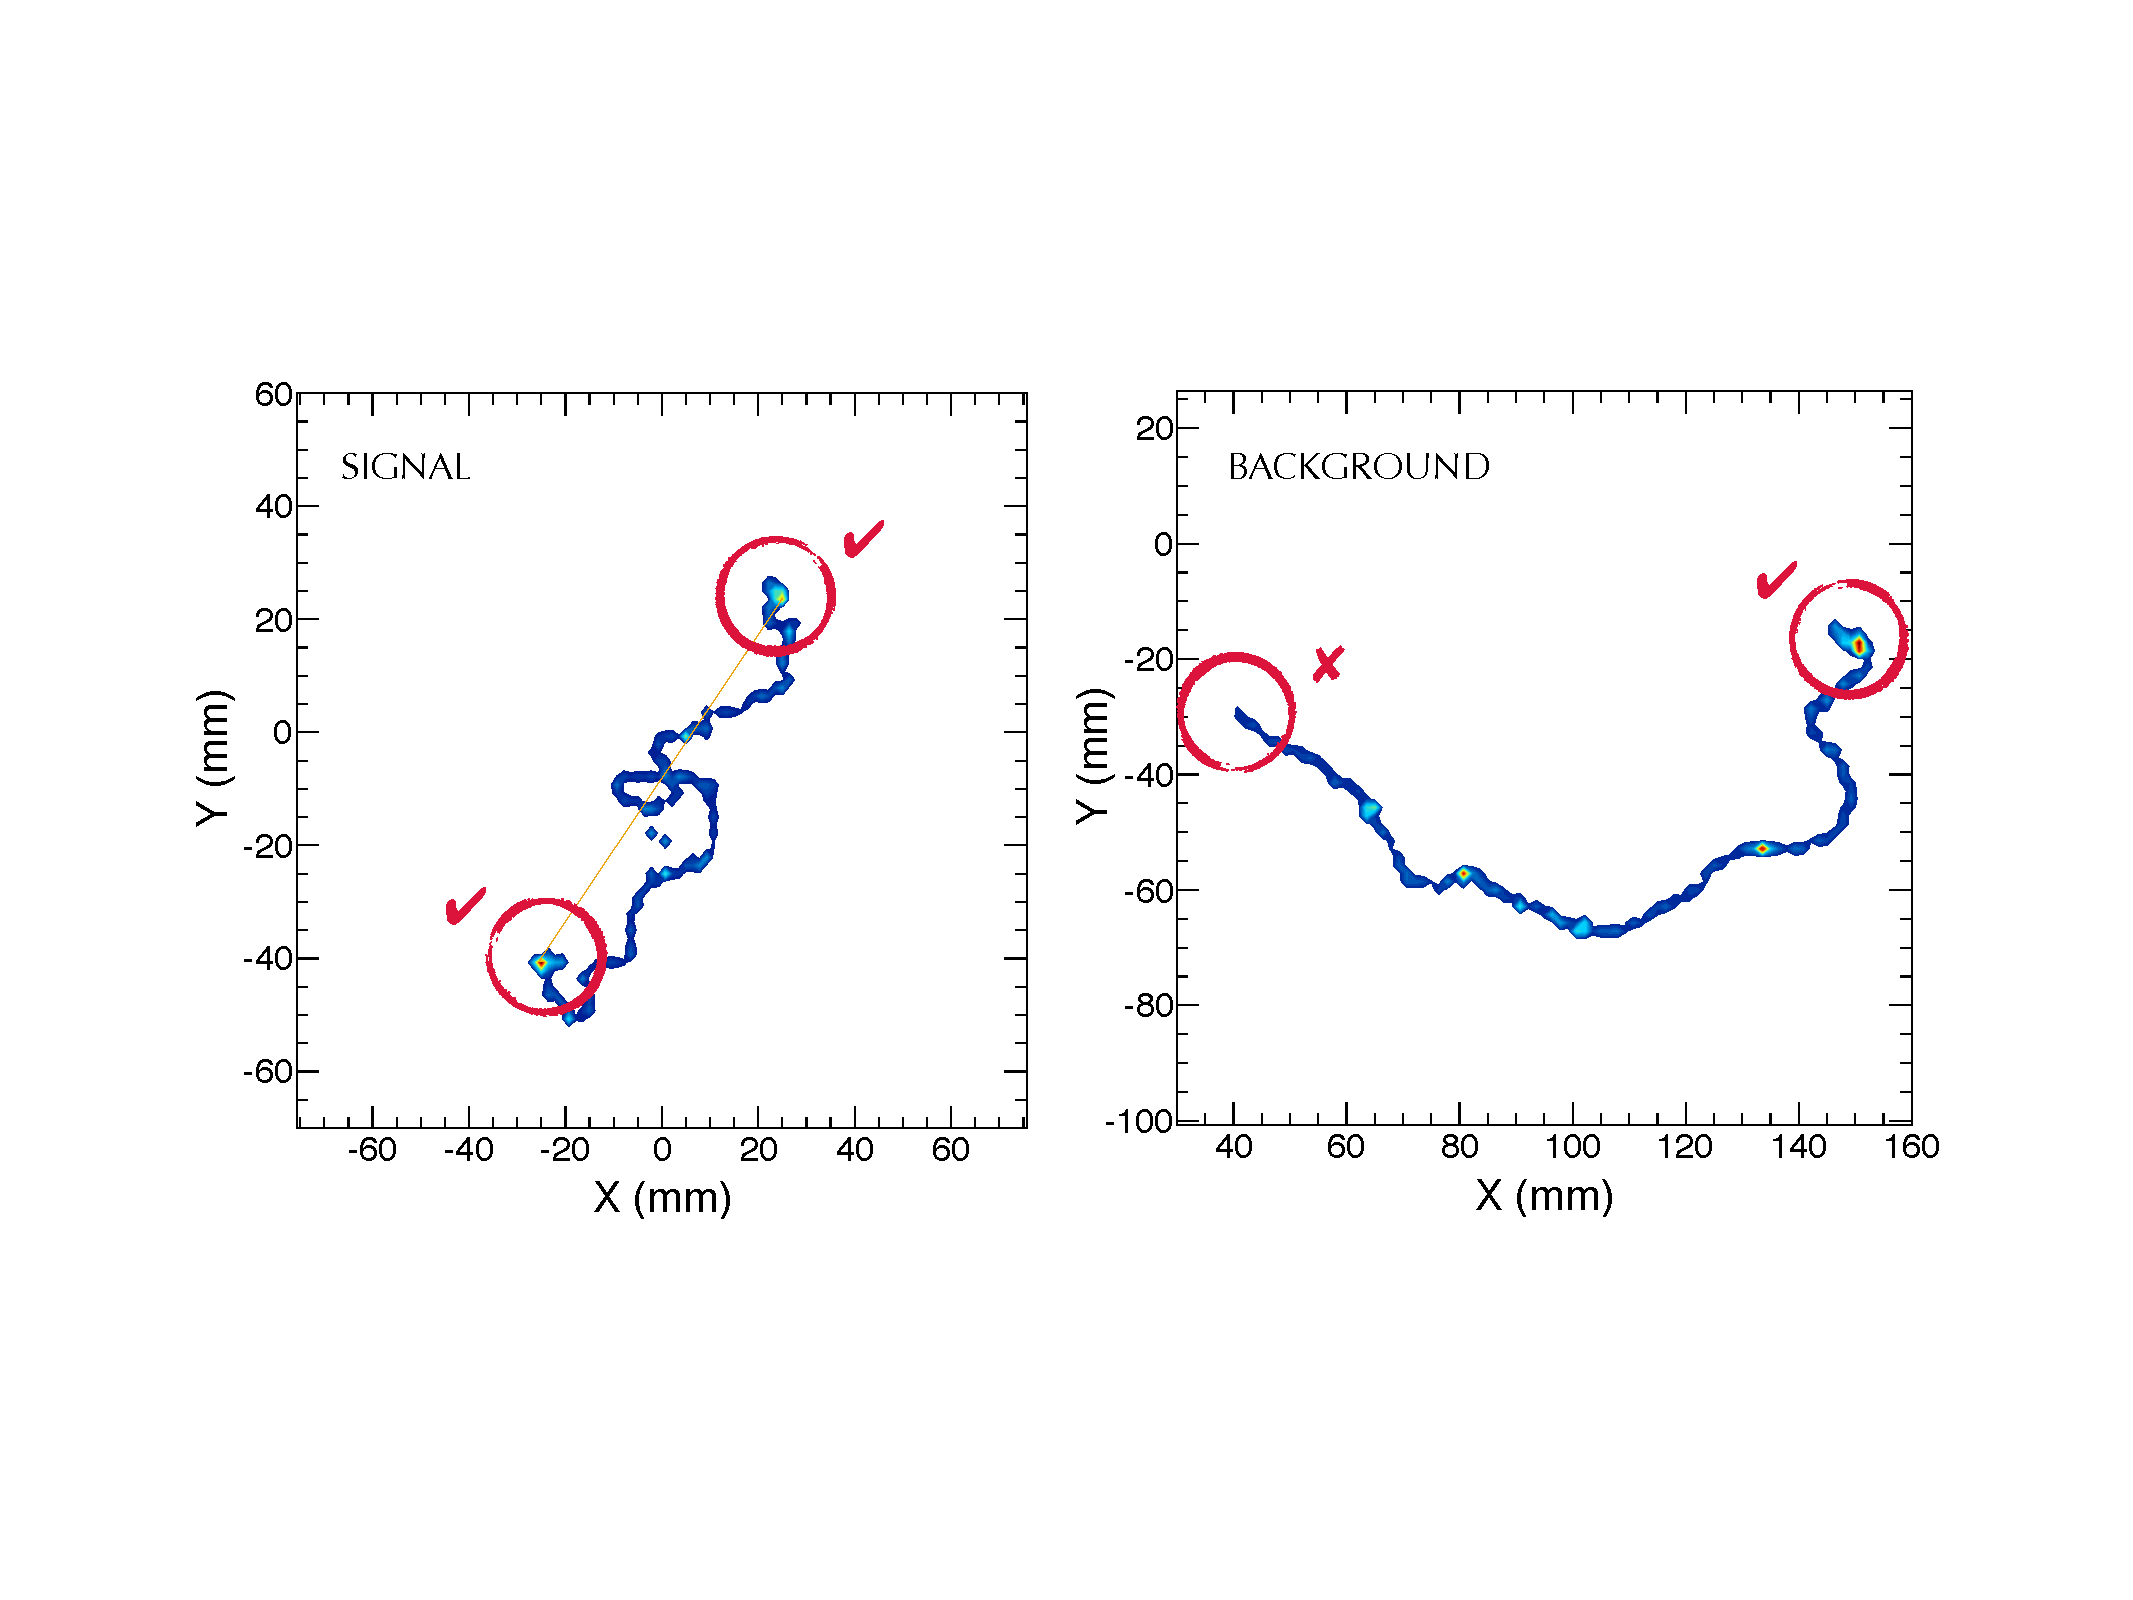
\includegraphics[width= 0.9\textwidth]{img/TrackSignature.pdf}
\caption{Monte Carlo simulation of a signal (\bbonu) event (left) and a  background event (right) in xenon gas at 15~bar. The color codes energy deposition in the gas. The signal consist of two electrons emitted from a common vertex, and thus it features large energy depositions  (blobs) at both ends of the track. Background event are, typically, single-electron tracks (produced by photoelectric of Compton interactions of high energy gammas emitted by \BI\ or \TL\ isotopes), and thus feature only one blob.} \label{fig.ETRK2}
\end{figure}
%%%%%

%%%%%
\begin{figure}
\centering
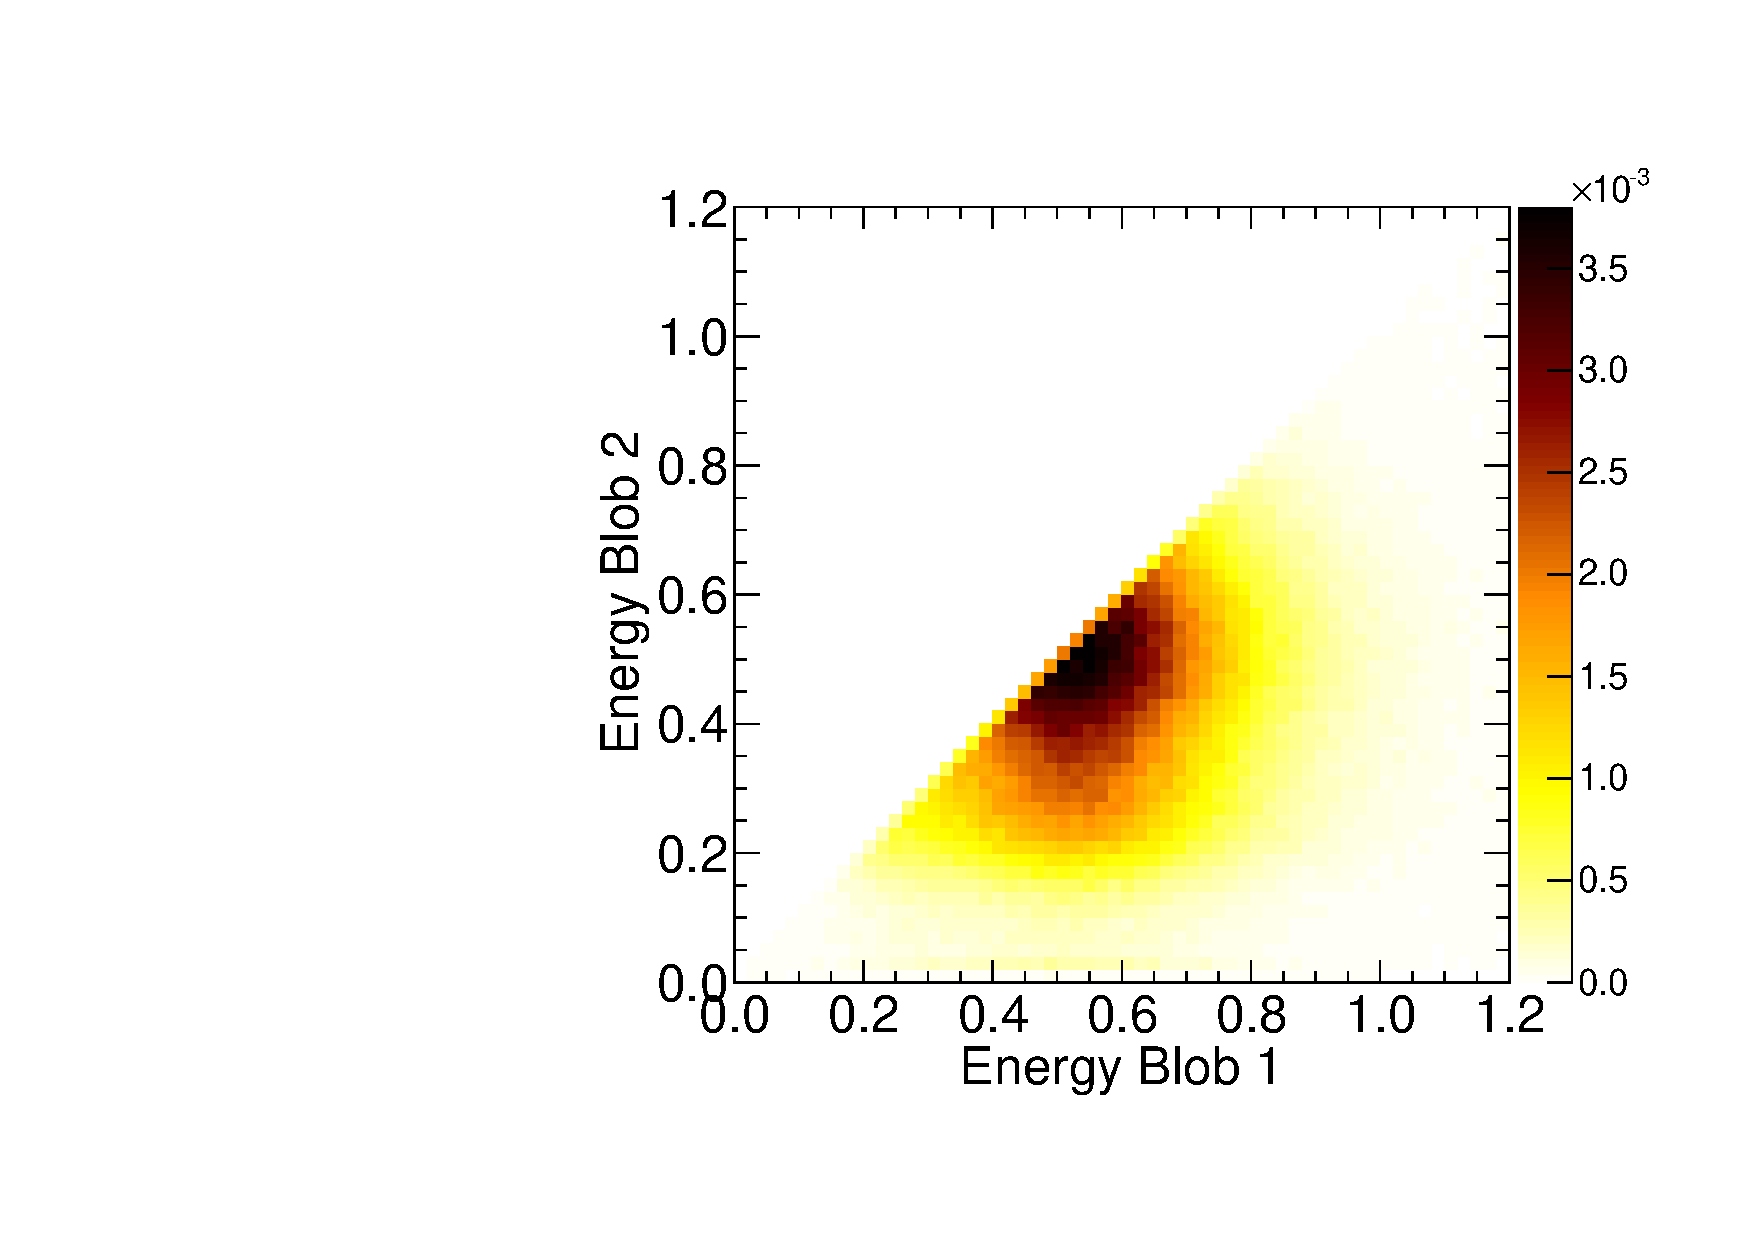
\includegraphics[width=0.45\textwidth]{img/EnergyBlobsSignal.pdf}
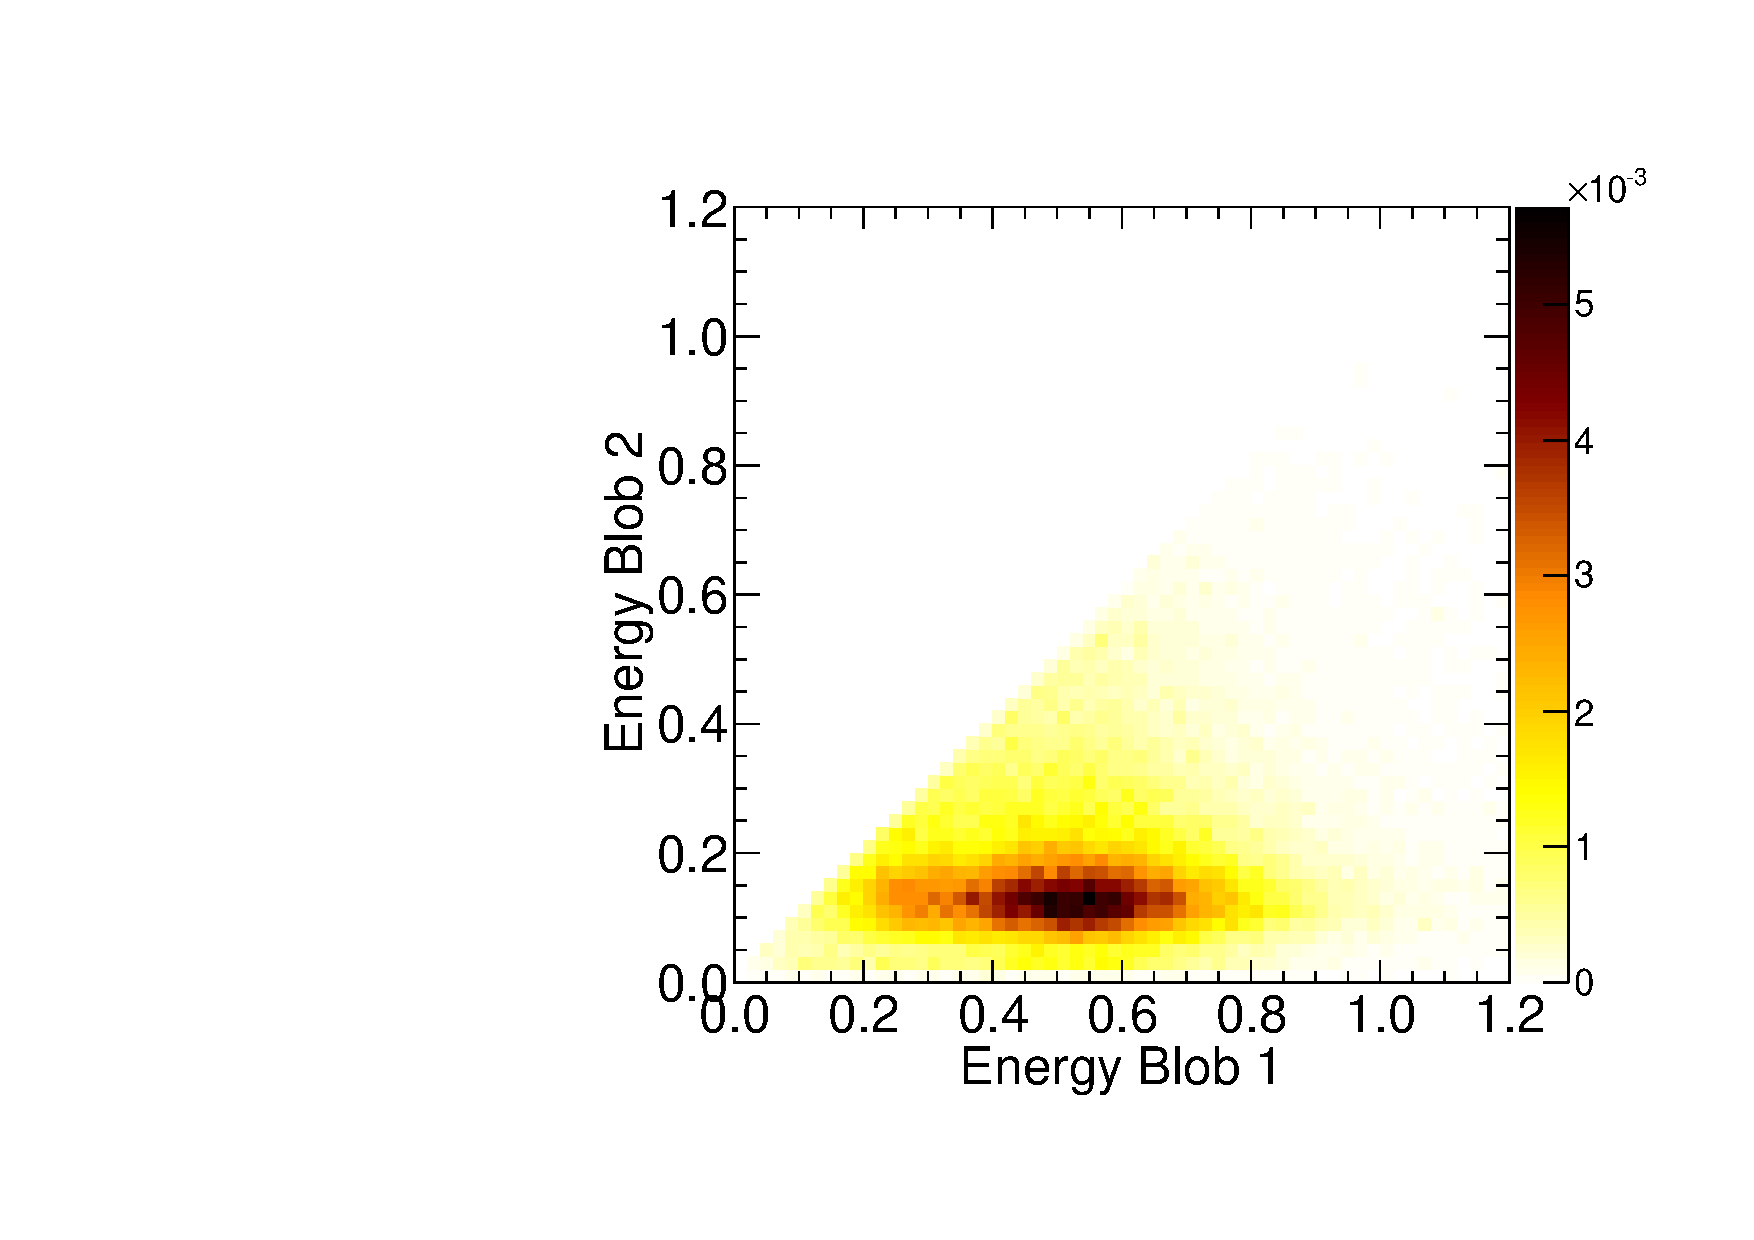
\includegraphics[width=0.45\textwidth]{img/EnergyBlobsTl208.pdf}
\caption{Probability distribution of signal (left) and background (right) events in terms of the energies of the end-of-track blobs. The blob labelled as `1' corresponds to the more energetic one, whereas `blob 2' corresponds to the less energetic of the two. In a signal event, the blobs have, in average, the same energy. In a background event, blob 1 has the same energy than a signal event while the energy of blob 2 is very small.} \label{fig.BLOBS}
\end{figure}
%%%%%

In addition of excellent energy reconstruction, NEXT has a topological signature, not available in most \bbonu\ detectors. 
Double beta decay events leave a distinctive topological signature in HPXe: a continuous track with larger energy depositions (\emph{blobs}) at both ends due to the Bragg-like peaks in the d$E$/d$x$ of the stopping electrons (figure \ref{fig.ETRK2}, top left). In contrast, background electrons are produced by Compton or photoelectric interactions, and are characterised by a single blob and, often, by a satellite cluster corresponding to the emission of 30-keV fluorescence X-rays by xenon (figure \ref{fig.ETRK2}).
Reconstruction of this topology using the tracking plane provides a powerful means of background rejection, as can be observed in Figure \ref{fig.BLOBS}. 

\subsection{NEXT background model}

 The major sources of background can be found in the 
radioactive contaminants in detector materials, in particular \BI\ and \TL\ isotopes.
The decay of \BI\ emits a number of de-excitation gammas with energies above 2.3 MeV. The gamma line at 2447 keV, of intensity 1.57\%, is very close to the $Q$-value of \XE. The gamma lines above \Qbb\ have low intensity and their contribution is negligible. 
The decay of \TL\ emits a de-excitation photon of 2614 keV with a 100\% intensity. The Compton edge of this gamma is at 2382 keV, well below \Qbb. However, the scattered gamma can interact and produce other electron tracks close enough to the initial Compton electron so they are reconstructed as a single object falling in the energy region of interest (ROI). Photoelectric electrons are produced above the ROI but can loose energy via bremsstrahlung and populate the window, in case the emitted photons escape out of the detector. Pair-creation events are not able to produce single-track events in the ROI. 

Radon constitutes also dangerous source of background due to the radioactive isotopes $^{222}$Rn (half-life of 3.8\,d) from the $^{238}$U chain and $^{220}$Rn (half-life of 55\,s) from the $^{232}$Th chain. As a gas, it diffuses into the air and can enter the detector. \BI\ is a decay product of $^{222}$Rn, and \TL\ a decay product of $^{220}$Rn. In both cases, radon undergoes an alpha decay into polonium, producing a positively charged ion which is drifted towards the cathode by the electric field of the TPC.  As a consequence, $^{214}$Bi and $^{208}$Tl contaminations can be assumed to be deposited on the cathode surface. Radon may be eliminated from the TPC gas mixture by recirculation through appropriate filters. There are also ways to suppress radon in the volume defined by the shielding. 

A detailed discussion of the NEXT background model can be found in \cite{Nebot-Guinot:2014raa}.

The excellent resolution of NEXT (0.5-0.7 \% FWHM), and the combination of a low radioactive budget with a topological signature (which yields an expected background rate of $5 \times 10^{-4} \ckky$), will allow the NEXT-100 detector to reach a sensitivity to the \bbonu\ period of $\Tonu > 7 \times 10^{25}$~yr for a exposure of 300 kg$\cdot$yr. This translates into a \mbb\ sensitivity range as low as $[67-187]$~meV, depending on the NME.

The detector is expected to start data taking in 2017. Currently, the first phase of the experiment, called NEW is being commissioned at the Canfranc Underground Laboratory (LSC), in Spain, and will start data taking later in 2015.
 

\section{BEXT: A HPXe TPC Operating in a Magnetic Field}

\subsection{Economy of Scale in a HPXe TPC}

\begin{figure}
\centering
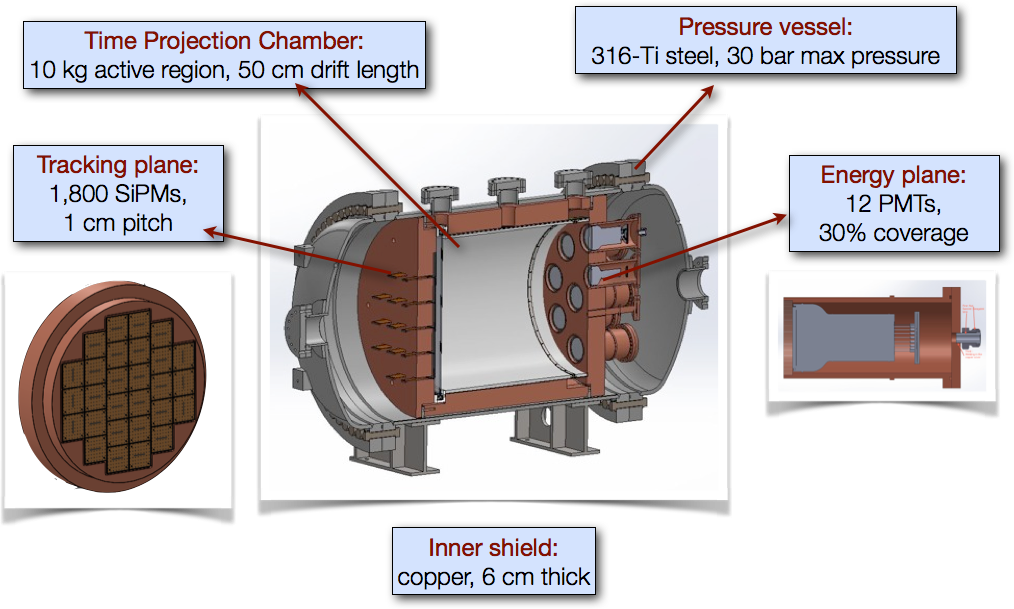
\includegraphics[width=0.9\textwidth]{img/NEW.png}
\caption{\small The NEW detector, currently being commissioned at the LSC (Canfranc, Spain).} \label{fig.NEW}
\end{figure}

The NEW detector, shown in Figure \ref{fig.NEW}, is the first phase of the NEXT experiment. The fiducial volume is a cylinder of 50 cm diameter and 60 cm length. The fiducial mass, at a pressure of 15 bar is 10 kg. The tracking plane has about 2,000 SiPMs, while the energy plane deploys 12 PMTs.

The fiducial volume of NEXT-100 (Figure \ref{fig.NEXT100}) is a cylinder of 110 cm diameter and 1200 cm length. The fiducial mass, at a pressure of 15 bar is $\sim$100 (98.5) kg. The tracking plane has about 9,000 SiPMs, while the energy plane deploys 60 PMTs.

The comparison between the first and the second phase of the NEXT experiment reveals clearly that a HPXe TPC benefits from the so-called {\em economy of scale} law, which in turn is a simple consequence of the fact that an HPXe is an homogeneous detector with a target mass ($M$) proportional to the fiducial volume (FV). If one approximates the FV by a cube of length $L$, then, doubling $L$ ($L \rightarrow 2 L$) results in multiplying the surface by 4 ($4 L^2$) and the volume by 8 ($8 L^3$). On the other hand, both the sensors need to instrument the apparatus and the backgrounds are roughly proportional to the detector surface, while the target mass (and therefore the signal) is proportional to the detector volume. Therefore the ratio signal to background (S/B) (and the cost of instrumentation versus the cost of the isotope) decreases linearly with $L$. In a detector without economy of scale (e.g. a detector built by repeating modules, such as the Germanium arrays), neither S/B nor the relative cost of instrumenting the system improve as the target mass increases. 

Indeed, both NEW and NEXT-100 are cylinders of near 1:1 aspect ratio (the diameter of the cylinder, $D$ is only slightly larger than the cylinder length $L$). Then, denoting $D_{NEXT}, L_{NEXT}, M_{NEXT}$~to the diameter, length and fiducial mass of NEXT-100 and $D_{NEW}, L_{NEW}, M_{NEW}$~to the diameter, length and fiducial mass of NEW, we find that doubling the NEW diameter (plus a 10\%), $D_{NEXT} = 1.1 \times 2 \times D_{NEW}$, and doubling the NEW length $L_{NEXT} = 2 \times L_{NEW}$, one increases the fiducial mass by one order of magnitude $M_{NEXT} = 10 \times M_{NEW}$, and the number of sensors by a factor 2 (plus a 10\%). 

The recipe to increase the fiducial mass to one ton is, then, appears straight forward: repeating the recipe:
we find that doubling the NEXT-100 diameter (plus a 10\%), $D_{BEXT} = 1.1 \times 2 \times D_{NEXT} \sim 2.4$~ m, and doubling the NEXT length $L_{BEXT} = 2 \times L_{NEXT} =2.4$~m, one increases the fiducial mass to almost one ton $M_{BEXT} = 954$~kg. To instrument the detector one would need about 45,000 SiPMs in the tracking plane (and about 250 PMTs in the energy plane). The naive ``economy of scale'' extrapolation law would predict that such a detector (if instrumented with the same sensors and materials than its predecessor and operating in the same environment) would have roughly a factor 2 less background events per year in the ROI.

\subsection{Operation in a magnetic field}
On the other hand, operation inside an intense magnetic field excludes the use of conventional PMTs, which must be replaced by sensors capable of providing a similar performance, to guarantee the excellent energy resolution characteristic of an HPXe.

Fortunately, a solution exists, already with today's technology. During the last five years, SiPMs have improved their performance in three crucial aspects: a) voltage operation uniformity; b) gain uniformity; and c) dark current.  
For example, SENSL manufactures large area SiPMs ($3 \times 3$~mm$^2$), capable of operating within 125 mV of the nominal voltage, with very small (< 0.5\%) gain spread and few ($\sim 2$) dark counts per photoelectron and micro-second. (REFERENCE?). This opens the possibility that the PMT energy plane is replace by an array of large area SiPMs. 

On the other hand, as will be discussed with detail in section XX, the additional separation power between signal and background attainable with a magnetic field deteriorates with pressure. In our studies, the optimal pressure is found to be 5 bar, but 10 bar provides an acceptable performance. Decreasing the operating pressure, on the other hand, requires an increase in the detector dimensions. Increasing both the diameter and the length to 3 m,
$D_{BEXT} = 3$~m, $L_{BEXT} = 3$~m, one obtains a fiducial mass of 1.2 tons. 

The studies discussed in section XX, also show that the separation between signal and background improves with the point resolution that can be achieved when reconstructing the electrons. Point resolution, in turn, depends of the diffusion in the electron drift and of sensor pitch. In pure xenon, diffusion is large, with typical values of 10 mm (for lateral diffusion) and about 5 mm (for longitudinal diffusion) after a typical drift of 1 m. However, as demonstrated recently by the NEXT collaboration (REF), the addition of very small quantities of a suitable additive (for example 0.1 \% of CO$_2$) reduces both the lateral and longitudinal dimensions to $\sim$ 1--2 mm, while having essentially no impact in the energy resolution. Therefore, BEXT will need to operate with such an additive. 

The SiPM pitch in the tracking plane of NEXT-100 is 10 mm (the sensors themselves are squares of 1 mm$^2$~surface). The minimum point resolution that is achieved in such a configuration is $10/\sqrt(12) = \sim 3$~mm (in practice the resolution is better, since the light emitted in the EL region is shared by more than one pixel, and thus one can reconstruct the position using a weighted procedure such as barycenter) which is much better than the resolution introduced by diffusion. On the other hand, in BEXT the resolution due to diffusion can be reduced to about 1--2 mm. Reducing the tracking plane pitch to 5 mm would result in a minimum resolution of 1.5 mm ($5/\sqrt(12)$). In practice light-sharing may provide a point resolution of 1--2 mm even with the larger pitch. The number of SiPMs needed for the BEXT tracking plane if the pitch is kept at 10 mm will be about 70 k, and about 280 k if the pitch is reduced to 5 mm. On the other hand, manufacturing a large quantity (e.g. 300 k) of SIPMs at very moderate costs (e.g. 3 \$/piece) appears feasible already today, resulting in a reasonable cost for the BEXT tracking sensors ($\sim 1$ M \$).  

The SiPMs making up the energy plane will have a surface of 3 mm$^2$, which appear as a good compromise between sensor area (which must be maximized to increase light collection) and dark current (which is proportional to the area of the sensor and must be kept within a reasonable value). The sensors will be located at a pitch of 10 mm, and Winston cone of outer radius 10 mm and inner radius 3 mm will focus the light in the sensors. Therefore, about 70 k pieces will be needed, at a cost that will probably not exceed 350 k\$. 

\subsection{BEXT conceptual design parameters}
The parameters of BEXT are summarized in Table \ref{tab.BEXT}. As will be shown in section XX the optimal performance for a pressure of 10 bar is achieved with a magnetic field of 0.5--0.7 Tesla. 
\begin{table}[htdp]
\caption{Parameters of BEXT}
\begin{center}
\begin{tabular}{|c|c|}
Parameter & Value \\
Magnetic field & Solenoidal, 0.5--0.7 Tesla \\
Operating pressure (bar) & 10 \\
Fiducial Volume & Cylinder of 21.1 m$^3$\\
Radius (m) & 1.5 \\
Drift Length (m) & 3 \\
Fiducial Mass (ton) & 1.2 \\
Tracking Plane & \\
Size of SiPMs (mm$^2$) & 1 \\
Pitch & 5 mm \\
Number of SiPMs & 280,000 \\
Energy Plane & \\
Size of SiPMs (mm$^2$) & 9 \\
Pitch & 10 mm \\
Number of SiPMs & 70,000 \\
\end{tabular}
\end{center}
\label{tab.BEXT}
\end{table}%
  



%As will be discussed with great detail later in this paper, the use of a magnetic field adds an extra handle to the topological signature, illustrated in Figure \ref{fig.KF}. 
%In the presence of a uniform external magnetic field $B$, charged particles spiral around the field lines in circular motion with radius $r = p_T/eB$, where $p_T$~ is the momentum of the electron transverse to the direction of the field and $e$~ is the electron charge. In the absence of multiple scattering, a single energetic electron produces a  single spiral with radius indicative of its momentum, and a double-electron track with the same energy will produce two spirals each with much less momentum and originating from a common vertex. This information can be used to provide an additional way of separating single-electrons arising from background processes from double electrons produced in \bbonu\ decays.
%However, in a dense medium such as xenon at high pressure, multiple scattering enters the picture, altering the electron trajectories and making it harder to distinguish signal from backgrounds. 
% 
% Figure \ref{fig.KF} illustrates the discussion. The top-left panel shows two electrons emitted in a \bbonu\ decay in the absence of magnetic field. Notice that the vertex where both electrons originated cannot be easily measured due to multiple scattering. However, the presence of two electrons is revealed by the two blobs at the end of the tracks (regions with higher density of hits and energy deposition, which originate when each one of the electron ranges out). Instead, the top-right panel shows a single background electron, which originates inside the detector when a photon, emitted by the decay of the isotope \BI\ enters the chamber and suffers a photoelectric interaction. Notice that the single electron only displays one blob in one of the vertexes. 
%
%When a sufficiently intense magnetic field is added, the separation between single and double electrons is strongly enhanced. The bottom-left panel shows again two electrons emitted in a \bbonu\ decay, turning in a magnetic field of 0.5 Tesla. The trajectory ``remembers'' that which would be followed in the absence of multiple scattering  (two helices originating from a common vertex). The bottom-right panel shows a single background electron turning in a 0.5 T magnetic field, following a single helix. This information can be used to enhance signal-background separation (see section XXX) {\em only if} a reasonable point-resolution (few mm at most) is achieved in the measurement of the track coordinates. To achieve such resolution, one needs to add to the xenon an additive capable of reducing diffusion while preserving the excellent energy resolution of characteristic of an EL TPC. The NEXT collaboration has studied several potential additives such as TMA (Diego paper), CH4 and O2. 
%   
% 
% The current (estimated) rejection factor for NEXT-100 is 0.5 counts per ton and keV in a year. If a resolution of \Qbb\ of 0.5 \% FWHM is confirmed in the large detector as we expect, this translates into 5 counts per ton in the ROI. The addition of a magnetic field may yield a value of 0.5-1 counts per ton in the ROI, thus allowing the HPXe technology to operate in the ton regime without being background limited. 
%
%
%
%


 


 
\section{MIST: A Magnetic Ion Selenium TPC}
\subsection{SeF$_6$~ as an alternative to \XE}

\SE\ has a \Qbb\ of 2995 keV and a natural abundance of about 9.2\%, making it a very attractive \bbonu\ candidate.  \SE\ has been studied by the NEMO experiment and is the isotope of choice for the Super-NEMO demonstrator, where a thin target sheet made of \SE\ is surrounded by a tracker and a calorimeter, immersed in a weak magnetic field. Alas, the Super-NEMO technology cannot be extrapolated to the ton scale. Alternatively consider selenium hexafluoride, SeF$_6$. This is a gas at room temperature up to nearly 10 bars, and therefore one can imagine a high-pressure SeF$_6$~ chamber. Given that there is one atom of \SE\ for each 6 atoms of Fluorine, the \SE\ isotope mass corresponds to about half of the SeF$_6$~mass. On the other hand, the average $Z$~ of the SeF$_6$~molecule is $(6 \times 9 + 34)/7 \sim12$, a factor 4.5 smaller than the $Z$~of xenon. Moliere  theory establishes that multiple scattering is proportional to Z, thus one can expect four times less multiple scattering in SeF$_6$~than in xenon and about 2 times less error associated to coordinate measurement (since measurement error goes with the square root of $Z$).  SeF$_6$~ is, however, highly electronegative, and, unfortunately, rather toxic, a feature that will, surely, complicate the feasibility of the scenario considered here.

\subsection{Detection: Ionization Imaging}

A TPC is essential to provide the track quality needed. However, due to its high electronegativity, SeF$_6$~makes impractical any attempt to realize well-behaved avalanche gain. In the absence of free electrons, no electroluminescence can be expected either.  In the presence of a substantial external electric field, free electrons might have a mean survival time sufficient that the cation-electron track images separate quickly on a scale corresponding to Onsager capture radius, before the symmetric pair of cation-anion images are formed. In the absence of recombination (whose existence or not must be determined experimentally), we assume, for this discussion, that recombination can be neglected.  

Any source of ionization, including \bb\ decay, thus leads to two track images with equivalent information moving in opposite directions: one cation track and one anion track. Detection of both track images can improve energy resolution, perhaps by $1\sqrt(2)$.  In any case, though, detection of both images is essential for placement of the event within the TPC active volume.   

With the requirement of 3-D imaging, and in the absence of avalanche gain, one is left to consider ultra-low-noise direct detection of ionization as proposed in REF (In 2007 I published a paper, "Ionization Imaging–A New Way to Search for 0ν-ββ ") based on pixelized detection of charge in a gaseous TPC.  The idea is to arrange the anode plane as a set of macroscopic pixels to collect charge with high efficiency, but without any avalanche gain. One condition to be met is to size the pixel sufficiently small that nearly all track topologies are captured with sufficient accuracy and clarity, but not so small that signal/noise is unfavorable.  Even if S/N were not a problem, diffusion places a lower limit on the physical size of pixels. For the ions of interest here, thermal rms diffusion after a meter drift is on the order of 1 mm, so a pixel size of 5 mm would be sufficient. This results in about 280 k pixels in each readout plane for a cylindrical fiducial volume of $R=1.5$~m (see discussion in previous section). We assume that energy resolution should not be worst than what can be achieved in a HPXe TPC.   

Typical ionic drift velocity is around 1 mm/ms, suggesting the need for sampling at 0.5 ms to capture the profile of arriving charge. However, CMOS image/charge sensing has a noise sweet spot in shaping time in the range of 10 - 100 $\mu$s.  Since only single channel optimization is relevant here, it may be possible to stretch shaping out to 500 $\mu$s without a very large increase in noise.  The power/real estate constraints imposed in multi-pixel circuitry can be easily relaxed, and a process that includes JFETs should help. About six samples in time would be needed for tracks lying mainly in the x-y plane. With six samples in time for each of 60 --100 spatial samples, the total number of samples would be around 480. In that case, the total noise budget of 480 electrons rms implies an individual sample noise limit of (480)1/2 $\sim$ 22 electrons rms.  Although not directly applicable here, single channel devices with this noise level are commercially available.  It follows that low-noise performance might not lie outside the realm of possibility. This is enhanced by recent  
progress in CMOS devices.  The current design results for multi-pixel CMOS imagers suggest that a noise level of 0.39 electrons rms [REF] is possible.  

A possible solution for the readout pixel consists in a an array of 
tiny collection electrodes on the presenting surface of the dielectric; the grid is hidden---located on the other side of the dielectric surface.   The total capacitance at input of the exposed JFET electrode might be on the order of $\sim 1$~ fF.  The idea is that the resistivity of the dielectric is sufficiently high that charge on the surface has a very long lifetime relative to the arrival of charge from the TPC volume.  What this means is that if field lines exist that would cause charge to land on the surface, charge continues to arrive only as long as the field line exists in the gas. Eventually, all field lines in the dielectric terminate in surface charge. Field lines in the gas are deflected away.  In other words, the process equilibrates when a quasi-static distribution forms such that no field lines enter/leave the dielectric surface.   

In this scenario, free charge in the gas is guided toward the collection electrode. This process  requires time to reach electrostatic equilibrium after the drift field and grid potential are first turned on. The hidden grid should have some applied potential to help realize or maintain the desired field; this requires optimization. An external, movable, ionizing radiation source can be used to speed equilibration.  Because the equilibrium dielectric surface charge distribution is static, the imminent arrival of signal charge from events of interest does not induce changes in the distribution.  The hidden metallic grid dynamically supplies image charges as needed.

To summarize, the concept appears to provide small collecting electrode size, minimum capacitance, 
freedom from surface charge injection by the grid (but also good signal development due to the existence of the grid), and complete charge collection.  Of course, many questions remain such as: 
\begin{enumerate}
\item For a given stability requirement, what is the quantitative relationship between dielectric resistivity and current in the gas needed to sustain stability? 
\item How forgiving is this scenario against variations in dielectric resistivity or current?
\item In electrostatic equilibrium, if no field lines enter/leave the dielectric, does the grid need a potential different than the collection electrode? 
\end{enumerate}

\subsection{Backgrounds}
Like xenon, neither   
fluorine nor selenium have  long-lived energetic radioisotopes that would pose intrinsic background dangers. In practice the backgrounds sources to be dealt with are the same than in the case of \XE, that is electrons produced by \BI and \TL\  isotopes.  

On the other hand, the larger value of \Qbb\ for \SE\ implies that the photoelectric peak of \BI\ located at 2.445 MeV is not a significant source of background, which will be dominated by Compton electrons produced by gammas of higher energies. While a full background model for MIST needs yet to be computed, we believe that it is safe to assume that the background in the ROI will not be larger than for NEXT.   

\subsection{Detection: System Concept}

The detection system must collect both cation and anion images, both to the place the event in space, and to improve energy resolution.  The general scheme is shown in figure 3.  The detector is a cascade of symmetric TPCs, with readout planes operating at ±HV. Each TPC segment supports a drift length of about 1 meter.  The pressure vessel resembles a railroad tank car.  High temperature superconducting cable is wound around the exterior to provide a magnetic field.   At the ends of the pressure vessel, the TPC segments are either 1/2 length to permit operation at ground potential, or an insulating plate could replace the end segment.

The readout planes consist of dielectric planes with exposed JFETs, as elaborated above for design 3.  Considerable electronics is embedded behind the dielectric plane. To collect either the anion track image or cation track image, the readout plane is assumed to accept either polarity signal at run-time setup, realizing an identical design.  To meet or exceed noise goals, I assume that the challenges of Gigohm feed-back/reset resistor in the charge-sensitive amplifier can be met.  Subsequent signal shaping and processing includes a slow 2 - 5 kHz 12-bit ADC to permit accurate charge measurement.  The challenge of supporting mixed signal activity with miniscule electronic noise is clear.  Nearest-neighbor logic will be needed to include below-threshold ADC values needed to optimize offline integration of signal.  The power to operate each signal plane is transported through a multi-conductor HV connector, in the same way that conventional x-ray machines provide current at HV to operate the cathode filament. Digital communications and data transport is obviously done with fiber optics.  Altogether, the readout planes represent an interesting design opportunity. 

 
\acknowledgments

This work was supported by the European Research Council under the Advanced Grant 339787-NEXT and the Ministerio de Econom\'{i}a y Competitividad of Spain under Grants CONSOLIDER-Ingenio 2010 CSD2008-0037 (CUP), FPA2009-13697-C04-04, FPA2009-13697-C04-01, FIS2012-37947-C04-01, FIS2012-37947-C04-02, FIS2012-37947-C04-03, and FIS2012-37947-C04-04.

\bibliography{nextb}

% Still to consider:
% - how does lower b.g. translate to sensitivity?


\end{document}